\documentclass[a4paper, 11pt, notitlepage]{article}
\usepackage[brazil]{babel}
\usepackage[utf8]{inputenc}
\usepackage{graphicx}
\usepackage[backend=biber]{biblatex}
\usepackage[hmargin=2cm,vmargin=2cm,bmargin=2cm]{geometry}
\usepackage{booktabs}
\usepackage{lscape}   % páginas landscape avulsas
\usepackage{svg}   %utilizar figuras .svg
\usepackage{amsmath}  %pacotes para matemática, opções de indentação, e links
\usepackage{amssymb}
\usepackage{amsthm}
\usepackage{caption}
\usepackage{indentfirst}
\usepackage{float}
\usepackage{makeidx}
\usepackage{multirow}
\usepackage{lscape}
\usepackage{xcolor}
\usepackage[pdftex]{hyperref}
\hypersetup{colorlinks=true}
\usepackage{array}
\usepackage{booktabs}
\evensidemargin 0 cm   %margens
\oddsidemargin 0 cm
\setlength{\textwidth}{16 cm}


%novo tipo de ênfase
\newcommand{\omph}[1]{\textsc{#1}}
\newcommand{\sen}{\textrm{sen }}


\newtheorem{lema}{Lema }[section]
\newtheorem{teorema}{Teorema }[section]
\newtheorem{corolario}[teorema]{Corolário }
\newtheorem{definicao}{Definição }[section]
\newtheorem{postulado}{Postulado }[section]
\newtheorem{proposicao}{Proposição }[section]
\newtheorem{exemplo}{Exemplo }[section]
\newtheorem{exercicio}{Exercício }
\newcommand{\cart}{\times}
\newcommand{\ses}{\Longleftrightarrow}
\newcommand{\entao}{\Longrightarrow}
\newcommand{\e}{\wedge}
\newcommand{\ou}{\vee}
\newcommand{\vazio}{\varnothing}
\newcommand{\sobre}{\longrightarrow}
\newcommand{\N}{\mathbb{N}}
\newcommand{\Q}{\mathbb{Q}}
\newcommand{\R}{\mathbb{R}}
\newcommand{\Z}{\mathbb{Z}}
\newcommand{\C}{\mathbb{C}}
\newcommand{\M}{\mathcal{M}}
\newcommand{\Ha}{\mathcal{H}}
\newcommand{\Ob}{\mathcal{O}}
\newcommand{\cmod}[3]{#1 \equiv #2\textrm{ (mod }#3\textrm{)}}
\newcommand{\tq}{\textrm{ tal que }}
\renewcommand{\qedsymbol}{$\blacksquare$}
\newcommand{\dsum}{\displaystyle\sum}
\newcommand{\divg}[1]{\vec{\nabla} \cdot #1}
\newcommand{\rot}[1]{\vec{\nabla} \times #1}
\newcommand{\what}{\widehat}
\newcommand{\wtil}{\widetilde}
\newcommand{\bemol}{\flat}
\newcommand{\sust}{\sharp}
\newcommand{\grad}{\textrm{grad }}
\newcommand{\divi}{\textrm{div }}
\everymath{\displaystyle}
\newcommand{\destq}[1]{\textbf{\textcolor{red}{\LARGE #1}}}
\makeatletter %only needed in preamble
%\renewcommand\tiny{\@setfontsize\tiny{7pt}{10}} %alterar tamanho da fonte para tabela
\makeatother

\numberwithin{equation}{section}  %faz a numeração das equações depender da seção

% bibliografia
\bibliography{bibtex/peterson1996,bibtex/curry1995,bibtex/fiske1984,bibtex/jolivette1994,bibtex/luetzelschwab1983,bibtex/venkataramaiah1978,bibtex/TabRad_v1,bibtex/TabRad_v3,bibtex/TabRad_v2,bibtex/TabRad_v8,bibtex/TabRad_v5,bibtex/TabRad_v6,bibtex/TabRad_v7,bibtex/codata2014,bibtex/nist_absorption,bibtex/ruby1977,bibtex/gucker1971,bibtex/joyce1969}

\begin{document}
\title{Espectroscopia Gama\footnote{Este trabalho está licenciado sob a Licença Creative Commons Atribuição-CompartilhaIgual 4.0 Internacional. Para ver uma cópia desta licença, visite \url{http://creativecommons.org/licenses/by-sa/4.0/} ou envie uma carta para Creative Commons, PO Box 1866, Mountain View, CA 94042, USA.}}
\author{Ana Carolina Rodrigues RA 154599\\ Eduardo Silva de Luca RA 145911\\ Pedro Rangel Caetano RA 147650\\}

\maketitle

\begin{abstract}
Utilizamos um espectroscópio gama para investigar propriedades físicas das emissões de diversos radionuclídeos. Caracterizamos o sistema, composto por cintilador de NaI(Tl), fotomultiplicadora e sistema de aquisição conectado ao computador, efetuando a calibração e caracterização da resolução em energia do mesmo. Adquirimos espectros gama de diversas fontes comerciais e comparamos os fotopicos encontrados com os valores da literatura. Também estudamos o espalhamento Compton de elétrons no interior do cintilador, determinando para a massa do elétron o valor $m_e = 512 \pm 2$ keV/c$^2$, bem como a aniquilação de pares (utilizando o espectro do ${}^{22}$Na) e a absorção de raios gama pela matéria, tendo obtido o coeficiente de absorção do Alumínio $(\mu/\rho)_{Al} = 0.09 \pm 0.03$ cm$^2$/g e do Chumbo $(\mu/\rho)_{Pb} = 0.115 \pm 0.003$ cm$^2$/g. Também verificamos que a estatística das contagens registradas pelo espectroscópio é bem descrita pela distribuição de Poisson, e determinamos a idade de uma camisa de Tório, obtendo o valor de $2.2 \pm 0.1$ anos.
\end{abstract}

\section{\label{sec:intro}Introdução}
A emissão de radiação gama ocorre a partir do decaimento de núcleos instáveis, segundo a sua composição de nuclídeos, de forma a obter uma configuração mais estável para o núcleo. O decaimento gama ocorre pela liberação de um fóton pelo núcleo, em um processo análogo ao de emissão de luz pelos átomos. No entanto, a força nuclear forte atuante entre os núcleons é muito mais intensa e as distâncias envolvidas são pequenas, da ordem de $10^{-15}$ m. Resultando na liberação de fótons de alta energia, chamados raios gama, que estão na faixa de MeV. $
$

Podemos entender o núcleo através da quantização de estados de energia. Dessa forma, a energia dos raios gamas liberados são bem definidas. Podendo ser utilizadas para a calibração de detectores de partículas na região de MeV.$
$

Nesse experimento, objetivou-se a introdução à física nuclear, enfatizando as propriedades do detector a cintilação NaI(Tl), os decaimentos característicos e a interação da radiação gama com a matéria, tais como Efeito Fotoelétrico, Espalhamento Compton e Produção e Aniquilação de Pares. Além disso foi estudado o espectro gama de uma camisa de lampião contendo ${}^{232}$Th, a fim de explorar uma distribuição mais complexa de fotopicos.

\section{\label{sec:teoria}Teoria}
As fontes estudadas no presente experimento, apresentam a emissão de raios gama seguidos de decaimentos de núcleos radioativos por decaimento alfa $(\alpha)$, beta $(\beta-)$, pósitron $(\beta+)$ ou captura de elétron (EC). Os diagramas de níveis de energia a seguir (Figura \ref{fig:diagrama.niveis}) apresentam algumas dessas transições para as diversas fontes comerciais analisadas.

\graphicspath{{relatorio/}}
\begin{figure}[H]
\centering
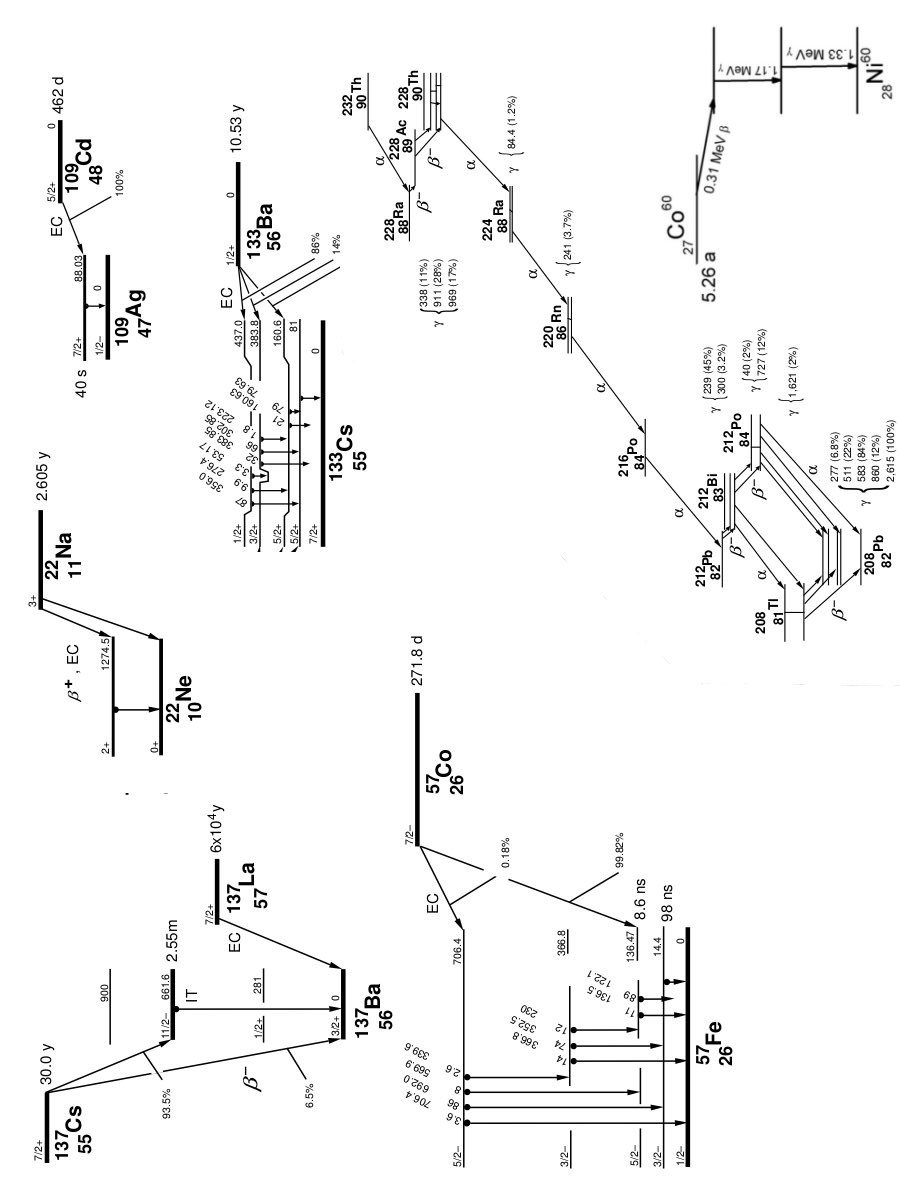
\includegraphics[scale=0.5]{fontes.jpg}
\caption{Diagrama de níveis de energia para diversas fontes comerciais, em sequência: Césio (Cs$^{137}$), Sódio (Na$^{22}$), Cádmio (Cd$^{109}$), Cobalto (Co$^{57}$), Bário (Ba$^{133}$), Tório (Th$^{232}$) e Cobalto (Co$^{60}$). Figura retirada de \cite{peterson1996}.}
\label{fig:diagrama.niveis}
\end{figure}

Os raios gama emitidos durante as transições no núcleo atômico interagem com o cristal de NaI, depositando toda sua energia no cristal, principalmente via efeito fotoelétrico (em energias menores que 1 MeV). De maneira geral, a passagem dos raios gama excita os átomos do cristal, ionizando seus elétrons, que irão produzir cintilações ao retornarem a seu estado fundamental.

O número de fótons detectados pode ser relacionado com a energia do raio gama original que excitou o material. A capacidade de emissão de cintilações para certos materiais ao serem cruzados por patículas carregadas é conhecida há muito tempo, sendo Rutherford o primeiro a usar ZnS em seus experimentos de espalhamento $(\alpha)$.

Ao interpretar o espectro de raio gama obtido é necessário um cuidado ao distinguir os picos devido a efeitos físicos acontecendo na matéria dos efeitos instrumentais. Um raio gama ao passar pela matéria interage, primeiramente, por efeito fotelétrico, espalhamento Compton e produção e produção de pares. A partir dessas interações, os raios gamas incidentes podem ser defletidos ou absorvidos pelo material. De tal forma que a quantidade de raios gamas remanescentes, N(x), depende da densidade atômica (p) do material e a espessura x do material atravessado segundo a equação:

\begin{equation}
 N(x) = N_{0}e^{-(\rho x)\mu\over\rho}
 \label{eq:absorcao.gamma}
\end{equation}

O coeficiente de atenuação linear, $\mu$, é uma constante de proporção em unidades de cm$^{-1}$. A razão $\mu\over\rho$ corresponde ao coeficiente de absorção de massa.

O Efeito Compton ocorre da colisão entre o fóton gama com um elétron atômico na qual a massa energia relativística e momento é conservado. Após a colisão o raio gama espalhado possui uma energia, E$_{\gamma'}$, menor que a sua original, E$_{\gamma}$, devido à transferência de energia para o elétron. Essas quantidades são relacionadas pela equação \eqref{eq:compton}
na qual $m_e c^2$ é a massa de repouso do elétron (511 keV) e $\theta$ é o angulo de deflexão do raio gama.
\begin{equation}
 \frac{1}{E_\gamma'} - \frac{1}{E_\gamma} = \frac{(1-\cos\theta)}{m_e c^2}
 \label{eq:compton}
\end{equation}

O elétron espalhado terá sua energia convertida no detector, de tal forma que a máxima energia, $E_{max}$, detectada decorre de uma colisão frontal ($\theta$= 180$^\circ$) entre o raio $\gamma$ e o elétron. $E_{max}$ corresponde portanto ao início do pico de Compton, seguido pela distribuição de energias menores possíveis desse mesmo efeito.

Logo após o pico de Compton, é possível distinguir um outro pico. Este ocorre devido aos fotons $\gamma$ que passaram direto pelo fotomultiplicador, interagiram com elétrons fora do detector. O raio gama espalhado pelo efeito Compton é detectado pelo fotomultiplicador, resultando no pico E$_{BS}$ (Backscttering). Por conservação de energia obtem-se que a massa de repouso do elétron segue a relação:

\begin{equation}
 m_e c^2 = \frac{2E_{\gamma}^{2} - 2E_{\gamma}E_{max}}{E_{max}}
 \label{eq:massaeletron}
\end{equation}

Um outro fênomeno observado é a produção e aniquilação de pares. A partir da aniquilação de um elétron negativo (partícula beta, $\beta-$) com um pósitron ($\beta+$), observa-se a emissão de dois fótons de 511 keV (raios $\gamma$) em direções opostas. Alguns núcleos radioativos decaem pela emissão de um pósitron.

O par elétron pósitron pode ser produzido quando um fóton com energia maior ou igual a duas vezes a massa de repouso do elétron (1022 keV) passa próximo a um núcleo. Em seguida o pósitron produzido irá aniquilar com outro elétron produzindo dois raios gamas de 511 keV. Dessa forma observa-se um pico de aniquilação em torno de 511 keV, seguido de um espalhamento Compton.

Pares elétron pósitron podem ser produzidos dentro do detector, e em seguida, se aniquilam. A aniquilação pode acontecer num período de tempo tão curto que os raios gamas emitidos se combinam resultando na energia do raio gama original (fotopico). No entanto, pode ocorrer de um ou dois gamas escaparem do detector sem interagir com o mesmo. O que resulta em um pico de escape, de energia 511 keV e 1022 keV abaixo do fotopico. Os picos de escape podem ser mais facilmente observados para raios gama com energias mais altas, sendo impossível que aconteçam para fótons com energia inferior a 1022 keV, naturalmente.

\section{\label{sec:metodologia}Metodologia}

\subsection{Instrumentação utilizada}
O contador de cintilações utilizado consiste em um cristal inorgânico de NaI (iodeto de sódio) dopado com átomos de Tálio (Tl), acoplado a um fotomultiplicador (PMT) cujo ânodo é conectado a um circuito eletrônico, funcionando como interface para o sistema de aquisição executado em um computador. Este sistema é ilustrado esquematicamente na Figura \ref{fig:esquema.cintilador}.

\graphicspath{{relatorio/}}
\begin{figure}[!htb]
\centering
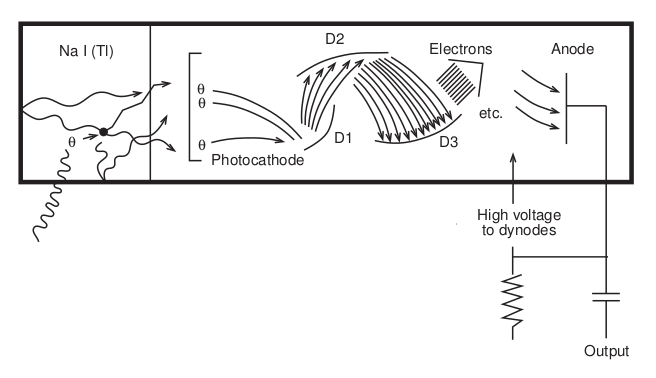
\includegraphics[scale=0.40]{cintilador.png}
\caption{Esquema do funcionamento do detector de cintilações, onde os fotoelétrons ejetados do fotocátodo são acelerador fotomultiplicador e a corrente amplificada é coletada no ânodo. Figura retirada de \cite{peterson1996}.}
\label{fig:esquema.cintilador}
\end{figure}

O sistema funciona da seguinte maneira: conforme descrito na seção anterior, cada fóton $\gamma$ que deposita sua energia no cristal acaba originando um pulso de fótons de curta duração. Estes fótons saem do cristal e incidem no fotocatodo da fotomultiplicadora, onde produzem uma pequena corrente de fotoelétrons emitidos por efeito fotoelétrico. Estes elétrons são acelerados por uma diferença de potencial e incidem sobre outro eletrodo, onde colidem e acabam arrancando um número maior de elétrons que são por sua vez acelerados em outro estágio da fotomultiplicadora, incidindo sobre outro eletrodo e produzindo uma corrente ainda maior. Este processo se repete algumas vezes, de forma que no ânodo da fotomultiplicadora ocorre um pulso com corrente proporcional à energia do fóton que interagiu com o cintilador. Por fim, a eletrônica acoplada ao ânodo da fotomultiplicadora converte o pulso de corrente para um pulso de voltagem, que é amplificado e tem sua amplitude mensurada por um conversor analógico digital (ADC) de 10 bits. Em suma, cada fóton incidente no cintilador origina um valor inteiro entre 0 e 1023, proporcional à energia deste fóton. Este valor inteiro é o que chamamos de canal da cintilação.

O sistema de aquisição possui dois modos de funcionamento distintos. O modo mais usado neste experimento é o Pulse Height Analysis (PHA), onde o sistema registra o canal correspondente a cada cintilação e produz uma contagem do número de cintilações registrado para cada canal. É possível também utilizar o modo Multichannel Scalling (MCS), onde o sistema conta o número de eventos detectados dentro de uma faixa de canais definida num intervalo de tempo determinado (\textit{dwell time}). Esta medição é repetida 1024 vezes, e o resultado é a sequência de contagens medida.

\subsection{Calibração}

Para que as medidas realizadas com este sistema sejam úteis é necessário calibrá-lo, obtendo a energia correspondente aos canais obtidos das cintilações. Para isto utilizamos as fontes de ${}^{22}$Na, ${}^{60}$Co, ${}^{54}$Mn e ${}^{109}$Cd. O ${}^{22}$Na é um $\beta^+$ emissor, portanto observamos um pico característico em $511$ keV, originário da aniquilação dos pósitrons emitidos pela amostra, e outro em $1274.5$ keV, devido à emissão $\gamma$ do núcleo durante a relaxação do mesmo após a emissão do pósitron. Como há uma chance não nula de dois fótons chegarem praticamente ao mesmo tempo no detector, ocorre de os pulsos gerados pelos dois fótons não serem corretamente discriminados pelo sistema de aquisição, e por isso observamos um outro pico na energia somada do elétron proveniente da aniquilação do pósitron e do fóton $\gamma$ emitido, isto é, $1785.5$ keV. Para o ${}^{60}$Co, ${}^{54}$Mn e ${}^{109}$Cd observamos linhas correspondentes a emissões $\gamma$ de $1173.23$, $834.85$ e $88.03$ keV.

Para cada uma das amostras adquirimos dados no modo PHA do sistema de aquisição até que o número de contagens nos canais nas regiões das linhas relevantes ultrapassasse 1000. O próprio programa de aquisição detecta as regiões correspondentes a picos nos espectros assim obtidos, fornecendo o centróide, FWHM e número de contagens naquela região. Selecionamos então as regiões correspondentes às linhas mencionadas anteriormente, e a cada uma dessas regiões ajustamos um perfil gaussiano somado uma baseline suposta linear na região da linha (conforme discutido em \cite{curry1995}), da forma

\begin{equation*}
  y = A \exp\left(\frac{-(x - \mu)^2}{\sigma^2} \right) + Bx + C,
\end{equation*}

\noindent onde $y$ é o número de contagens, $x$ o canal, $\mu$ e $\sigma$ o centro e desvio padrão da gaussiana e $A$, $B$ e $C$ definem a altura máxima da gaussiana e os parâmetros do baseline. Deste ajuste obtivemos portanto o canal correspondente ao centro da linha, com o erro associado. Utilizando os valores medidos do centro de cada uma das linhas das amostras usadas conjuntamente com os valores de referência da energia destas linhas (obtidos de\footnote{Estes valores estão disponíveis em \url{http://www.nucleide.org/DDEP_WG/DDEPdata_by_A.htm}} \cite{TabRad_v1,TabRad_v3,TabRad_v5,TabRad_v8}) ajustamos um polinômio de grau 2, que nos forneceu a correspondência entre canais e energias em keV.

\subsection{Espectros de fontes comerciais\label{sec:espectro.comercial}}
Uma vez obtida a calibração, podemos medir os espectros $\gamma$ de fontes quaisquer utilizando o modo PHA do sistema de aquisição e transformando os canais nos valores de energia associados. Também é possível obter os valores do centro e FWHM de cada linha utilizando o ajuste gaussiano com baseline previamente descrito, sendo o centro dado pelo parâmetro $\mu$ e o FWHM por $2.355 \sigma$. Utilizando a contagem na região da linha e os parâmetros do baseline naquela região podemos obter ainda a intensidade daquela linha em uma dada aquisição: se o intervalo de canais $[x_a, x_b]$ delimita a linha observada e $A_{baseline}$ e $A_{sinal}$ correspondem às áreas abaixo do sinal e do baseline ajustado, se $I$ é o número de contagens detectado na região da linha o número de contagens corrigido $I_{corrigida}$ é dada por

\begin{equation*}
  I_{corrigida} = I \cdot \frac{A_{sinal} - A_{baseline}}{A_{sinal}}.
\end{equation*}

Obtendo $A_{sinal}$ por integração numérica dos dados adquiridos e $A_{baseline}$ pela expressão, obtida por integração da expressão utilizada para a baseline,

\begin{equation*}
  A_{baseline} = B \frac{x_b^2 - x_a^2}{2} + C\left(x_b - x_a\right),
\end{equation*}

\noindent podemos encontrar o número de contagens corrigido de uma linha qualquer.

\subsection{Checagem da calibração}
Checamos a calibração de duas formas: primeiramente tomamos o espectro de uma fonte de ${}^{137}$Cs e comparamos o valor obtido para o centro da linha observada com o valor de referência presente na literatura. Também foi coletado o espectro gama para diversas fontes comerciais: Césio (Cs$^{137}$), Sódio (Na$^{22}$), Cádmio (Cd$^{109}$), Cobalto (Co$^{57}$), Bário (Ba$^{133}$), Manganês (Mn$^{54}$) e Cobalto (Co$^{60}$).  Medindo o canal correspondente ao centro de cada uma das linhas destes elementos e comparando a energia obtida com nossa calibração com a energia presente na literatura pudemos checar a precisão de nossas medidas.

\subsection{Resolução em energia}

A partir dos espectros obtidos anteriormente estudamos também a dependência da resolução do detector utilizado na energia. A resolução do detector corresponde à razão entre a largura das linhas observadas, $\Delta E$ e a energia da linha $E$, isto é

\begin{equation*}
  r = \frac{\Delta E}{E}.
\end{equation*}

É estabelecido na literatura referente a cintiladores de NaI(Tl) que a dependência na energia desta resolução segue a seguinte equação \cite{venkataramaiah1978}

\begin{equation}
 \frac{\Delta E}{E} = \frac{m}{E} + b
 \label{eq:resolution}
\end{equation}

Além disso, argumentos puramente estatísticos\footnote{Assumindo que as contagens seguem uma distribuição poissoniana na região da linha.} fornecem que

\begin{equation*}
  \Delta E \propto \sqrt{E}
\end{equation*}

\noindent portanto

\begin{equation*}
  \ln\left(\frac{\Delta E}{E}\right) = 0,5 \ln\left(E\right) + k
\end{equation*}

\noindent onde $k$ é uma constante a ser determinada.

Para checar estas relações, selecionaram-se os fotopicos de interesse nos espectros já obtidos, obtendo seus respectivos centros e FWHM conforme já descrito na seção \ref{sec:espectro.comercial}. Convertendo os valores em canais destes para keV usando a calibração obtida e considerando a largura da linha dada pelo FWHM obtivemos a resolução de cada linha medida. Com estes dados fizemos gráficos tanto da resolução vs. inverso da energia como do logaritmo natural da resolução pelo logaritmo da energia, realizando os ajustes lineares adequados.

\subsection{Espalhamento Compton}

Como discutido na seção \ref{sec:teoria}, o espalhamento Compton introduz alguns artefatos no espectro $\gamma$ de uma fonte qualquer. Normalmente aparecem na região com energia menor que a do fotopico duas estruturas. 

A primeira é um platô com uma queda súbita um pouco antes do fotopico. Esta queda súbita é conhecida como \textit{Compton Edge}. O que ocorre é que este platô observado é devido ao espalhamento Compton dos fótons $\gamma$ no cintilador, que depositam apenas parcialmente sua energia no elétron espalhado e escapam do detector. Ocorre que há uma quantidade máxima possível de energia obtida por um elétron após uma colisão elástica com um fóton, correspondente a um espalhamento frontal. Esta energia $E_{max}$ é precisamente a energia do Compton Edge. A partir da conservação de energia e da equação \eqref{eq:compton} é possível então deduzir a equação \eqref{eq:massaeletron}, e determinar a massa do elétron a partir desta informação

\begin{equation*}
 m_e c^2 = \frac{2E_{\gamma}^{2} - 2E_{\gamma}E_{max}}{E_{max}}
\end{equation*}

A segunda é um pico que aparece na região onde está o platô, com uma energia defina $E_{BS}$. Este pico é chamado de pico de \textit{backscattering}, e é devido ao retroespalhamento de fótons que passaram incólumes pelo detector em materiais próximos ao cintilador. Por razões geométricas, estes fótons retroespalhados normalmente espalharam em ângulos próximos a 180$^\circ$. Sua energia é portanto complementar à energia do Compton Edge:

\begin{equation}
  E_{BS} + E_{max} = E_{\gamma}  \label{eq:cons.energia.compton}
\end{equation}

É possível também determinar a massa do elétron a partir destas energias. Usando a expressão anterior na equação \eqref{eq:compton} descobrimos a expressão

\begin{equation}
  m_e c^2 = \frac{2E_\gamma^2}{E_\gamma - E_{BS}} - 2 E_\gamma
  \label{eq:massaeletron.bs}
\end{equation}


Neste experimento, coletamos o espectro gama das fontes de ${}^{22}$Na, ${}^{137}$Cs e ${}^{54}$Mn. Detectamos para estes espectros a localização do pico de backscattering e do Compton Edge. Procedemos da seguinte forma:

\begin{itemize}
  \item Para cada amostra, carregamos os dados e os calibramos
  \item Definimos uma região de observação contendo o fotopico e o pico de backscatter
  \item Suavizamos os dados (aplicando médias locais com pesos gaussianos) e calculamos a derivada numérica dos dados
  \item Encontramos o fotopico a partir do primeiro ponto onde a derivada deixa de ser positiva e se torna negativa.
  \item Obtivemos a incerteza do fotopico a partir da incerteza dos parâmetros da calibração. Esta é uma boa estimativa pois, como verificado durante a análise dos espectros de várias fontes comerciais, esta é a maior fonte de incerteza (sendo a incerteza obtida ao ajustar os picos tipicamente desprezível)
  \item Encontramos, analisando a derivada do sinal, o mínimo mais próximo do fotopico: esta é a energia do background do compton edge
  \item Encontramos a energia do platô do compton edge, encontrando o primeiro máximo da derivada à esquerda do mínimo compton determinado no passo anterior
  \item Seguindo \cite{jolivette1994}, encontramos o ponto onde a energia cai a uma fração de 54 \% da diferença de energia entre o platô e o background. Esta é a energia do compton edge $E_{max}$
  \item Ainda seguindo \cite{jolivette1994}, estimamos a incerteza na energia do compton edge como a variação da energia do compton edge quando variamos a fração de 50\% a 58\% (\cite{jolivette1994} argumenta, usando simulações de Monte Carlo da interação de fótons $\gamma$ com o detector, que este é o desvio padrão da fração utilizada).
  \item Com os valores obtidos para $E_{max}$, $E_{BS}$ e os valores tabelados de $E_{\gamma}$ encontramos a massa do elétron utilizando as expressões \eqref{eq:massaeletron} e \eqref{eq:massaeletron.bs}, com sua incerteza propagada associada.
  \item Por fim, calculamos a média, ponderada pelo inverso da variância, das diferentes massas obtidas, bem como o desvio associado.
  \begin{eqnarray*}
  \overline{m_ec^2} &= \sum_{k} (m_e c^2)_k \frac{1}{\Delta (m_e c^2)_k^2} \\
  \Delta \overline{m_e c^2} &= \left(\sum_{k} \frac{1}{\Delta (m_e c^2)_k^2}\right)^{-1/2}
  \end{eqnarray*}
  Calculamos também o $\chi^2$ normalizado pelo número de graus de liberdade desta medida,
  \[
  \chi^2 = \frac{1}{N-1}\sum_k\left(\frac{(m_ec^2 )_k - \overline{m_ec^2}}{\Delta (m_e c^2)_k}\right)^2
  \]
  \noindent que deve possuir valor próximo de $1$ e o desvio relativo ao valor padrão aceito pelo CODATA \cite{codata2014}, de 
  \[
  m_e c^2 = 510.9989461 \pm 0.0000031\text{ keV}
  \]
\end{itemize}

\subsection{Produção e aniquilação de pares}

No experimento de produção e aniquilação de pares foi coletado o espectro da fonte de ${}^{22}$Na por um tempo longo o suficiente para observar o pico de aniquilação dos pósitrons emitidos pela fonte.

Também captamos o espectro do ${}^{232}$Th, que possui uma linha gama com energia superior a $1022$ keV. Fótons com energia maior que este valor podem interarir com o detector por produção de pares, produzindo um elétron e um pósitron. O pósitron rapidamente é aniquilado, emitindo dois fótons de $511$ keV (a energia cinética do pósitron é muito pequena e pode ser desconsiderada). Ambos os fótons possuem uma chance de escapar do cristal de NaI(Tl). Quando um dos fótons escapa a energia do detector é $511$ keV inferior à energia do fotopico associado ao fóton $\gamma$ original, e quando os dois fótons escapam a energia é $1022$ keV inferior à energia do fotopico. Aparecem então linhas secundárias, do primeiro escape e segundo escape.

\subsection{Absorção de raios gama}

Foi investigada a absorção de raios gama por diferentes materiais, no caso o alumínio e o chumbo. 

Raios gamma (e X) tem uma probabilidade não-nula de interagir com a matéria, sofrendo espalhamento ou mesmo sendo absorvidos. Por esta razão, ao incidir radiação gama num material observamos que, a cada $N_0$ fótons incidentes, restam

$$ N(x) = N_0 e^{-(\rho x) \mu / \rho} $$

\noindent fótons após atravessar uma espessura $x$ do material. O produto $\rho x$ costuma ser denominado espessura, sendo medido em unidades de massa por comprimento ao quadrado. A razão $\mu/\rho$, por sua vez, é denominada \textit{mass attenuation coefficient}, ou apenas coeficiente de absorção.

Verificamos experimentalmente esta relação, detectando a radiação gama de uma fonte de ${}^{137}$Cs, na região da linha de 661 keV, que atravessou pequenas chapas de alumínio e chumbo de espessura variada. Foram utilizadas dez placas de alumínio com o parâmetro $\mu/\rho$ (espessura) variando entre 129 e 849 mg/cm$^{2}$, e quatro placas de chumbo entre 1230 e 7435 mg/cm$^{2}$. Fazendo um gráfico do logaritmo da taxa de contagens vs. espessura para cada um dos materiais conseguimos recuperar a taxa de contagens antes e o coeficiente de atenuação por um ajuste linear, pois

$$ \log \frac{dN}{dt}(x) = \log \frac{dN_0}{dt} - \frac{\mu}{\rho} \left(\rho x\right). $$

Para a análise

\begin{itemize}
\item Obtemos o número de \textit{net counts}, definido como o número de contagens na linha do ${}^{137}$Cs, descontadas as contagens correspondentes a um baseline linear entre os extremos da janela de observação que define a linha.
\item Obtemos o \textit{live time} registrado pelo programa de aquisição (tempo de aquisição descontado do tempo morto do detector)
\item Obtemos a taxa de contagens (\textit{net count rate}) dividindo \textit{net counts} por \textit{live time} para cada observação
\item Estimamos o erro de \textit{net count rate} como a raiz da razão \textit{net count rate} por \textit{live time} (verifique  comentários na seção \ref{sec:estatisticas.contagem} sobre a variância da taxa de contagens).
\item Fizemos o gráfico de log(\textit{net count rate}) por log(\textit{espessura}) e com um ajuste linear obtivemos o coeficiente de atenuação.
\end{itemize}

\subsection{Estatísticas de contagem \label{sec:estatisticas.contagem}}

Checamos também as estatísticas de contagem do detector usado. Para isso utilizamos o programa de aquisição no modo MCS com uma fonte de ${}^{137}$Cs e uma janela de observação na região da linha de 661 keV. Neste modo, o detector conta o número de eventos (cintilações) com energia dentro de uma faixa determinada (no nosso caso, a linha do Césio) ocorridos dentro de um intervalo de tempo chamado \textit{dwell time}. Este processo é repetido 1024 vezes, e com isto conseguimos dados sobre a distribuição do número de contagens obtidas neste tempo. No nosso caso, tomamos as medidas para 3 valores de \textit{dwell time}: 0.4, 4 e 10 s.

Sabe-se \cite{ruby1977} que a distribuição do número de partículas emitidas por amostras radioativas num tempo fixo é um processo binomial, que pode ser aproximado (quando o número de núcleos emitindo é muito grande e a probabilidade de decaimento de um dado núcleo no período de tempo observado é muito pequeno, mas o produto de ambos - o número médio de decaimentos - é finito) por uma distribuição poissoniana.

Outros processos aleatórios contribuem para a variância observada do número de contagens, envolvendo o processo de detecção da radiação no espectrômetro. A soma de todos estes processos é, tipicamente, poissoniana \cite{joyce1969}, i.e., a probabilidade de contarmos $k$ partículas num intervalo de tempo fixado $t$ é

$$ P(k) = e^{-\lambda} \frac{\lambda^k}{k!} $$

\noindent onde $\lambda$ é o valor esperado do número de contagens, $\lambda = \text{E} \left[ k \right]$. Além disso, a variância do número de contagens é, no caso de uma distribuição de Poisson, dada por $\text{Var}\left[k\right] = \lambda$.

Neste experimento estamos mais interessados nas distribuições das taxas de contagens, isto é, no número de contagens pelo tempo transcorrido. Sendo esta taxa dada por $A = \frac{k}{t}$, onde $t$ é o \textit{dwell time}, temos

$$ \text{E}\left[A \right] = \frac{\lambda}{t} $$
$$ \text{Var}\left[A \right] = \frac{\lambda}{t^2} = \frac{\lambda}{t} $$

Estimando a partir dos dados experimentais a média da distribuição como a média das taxas de contagens observadas $\left\langle A \right\rangle$ podemos também inferir que o desvio padrão da distribuição é

$$ \sigma = \sqrt{\frac{\left\langle A \right\rangle}{t}} $$

Com os dados brutos coletados podemos, portanto, observar o histograma das taxas de contagens para os valores de \textit{dwell time} utilizados. Apenas com a média da taxa de contagens obtida em cada uma das medidas podemos determinar a distribuição de Poisson adequada, já que o desvio padrão é dado pela equação acima. Fizemos então histogramas destes dados, superpostos a gaussianas com média e desvio padrão computados com a hipótese de que os dados são poissonianos (quando o número de contagens é grande tipicamente podemos transitar impunemente entre as distribuições gaussiana e poissoniana \cite{ruby1977, gucker1971}) e observamos, visualmente, um bom acordo entre o modelo e as medições.

\subsection{\label{sec:metodologia.torio}Camisa de Tório}

Foi obtido o espectro gama da camisa de lampião (Th$^{232}$) por um longo tempo de exposição (24 horas). Para esse mesmo período de tempo, foi coletado o espectro da radiação de fundo, a fim de comparar a contribuição das séries de decaimento do Tório para a radiação de fundo.

A partir destes dados obtivemos a idade da camisa de lampião. Para tanto, determinamos a razão entre as atividades do ${}^{228}$Ra e do ${}^{228}$Th na amostra. Segundo \cite{luetzelschwab1983}, a dependência desta razão no tempo é dada por

\begin{equation}
 r(t) = \frac{1 - e^{-\lambda_B t}}{1 - 1.5 e^{-\lambda_B t} + 1.5 e^{-\lambda_C t}}  \label{eq:razao.teorica}
\end{equation}

\noindent onde $B$ se refere ao ${}^{228}$Ra, $C$ ao ${}^{228}$Th, $\lambda$ é a constante de decaimento e $\lambda_B = 3.829 \cdot 10^{-9}$ s$^{-1}$ e $\lambda_C = 11.484 \cdot 10^{-9}$ s$^{-1}$ \cite{TabRad_v5,TabRad_v7}. Por outro lado, esta razão é igual à razão das atividades do ${}^{228}$Ac e do ${}^{212}$Pb \cite{peterson1996}. Esta última pode ser obtida experimentalmente pelo seguinte procedimento:

\begin{itemize}
 \item Primeiramente subtraimos o background dos dados obtidos para o tório e suavizamos os dados. Calibramos o espectro usando os parâmetros de calibração obtidos anteriormente.
 \item Selecionamos uma janela de observação entre 825 e 1100 keV. Esta região contêm dois picos do ${}^{228}$Ac, em 911 e 969 kev, e um pico do ${}^{208}$Tl, em 860 keV.
 \item Ajustamos uma função correspondente à soma de um baseline linear com três picos gaussianos

\begin{equation}
I(x) = ax + b + \sum_{k=1}^{3} \frac{A_k}{\sqrt{2\pi \sigma_k}} \exp\left(-\frac{(x - E_k)^2}{2\sigma_k^2}\right) \label{eq:tres.picos}
\end{equation}

 \item Obtemos a intensidade das linhas do Actínio na janela de observação como a integral das gaussianas centradas em $E_2$ e $E_3$ (correspondentes às linhas de 911 e 969 keV). Corrigimos também esta intensidade pela eficiência relativa\footnote{Note que embora não saibamos a eficiência de fato ($\epsilon(E)$ é a eficiência relativa à eficiência em 240 keV), ela não é necessária, já que computaremos a razão entre as atividades dos dois isótopos.} em energia do detector, $\epsilon(E)$, dada por

\begin{equation}
\epsilon(E) = 62 \left(\frac{E}{240}\right)^{-1.648} \label{eq:eficiencia}
\end{equation}

\noindent (eficiência relativa à eficiência em 240 keV). A intensidade das emissões do Actínio na janela de observação é dada portanto por

\begin{equation} i_{Ac} = \frac{A_2}{\epsilon(E_2)} + \frac{E_3}{\epsilon(E_3)}  \label{eq:i_Ac}
\end{equation}

 \item Obtemos dos dados padrão tabelados para o ${}^{228}$Ac a probabilidade de uma transição aleatória deste ocorrer na janela de observação usada, $p_{Ac}$. Estimaremos então a atividade total do Actínio como

\begin{equation}
 I_{Ac} = \frac{i_{Ac}}{p_{Ac}}  \label{eq:I_Ac}
\end{equation}

 \item Selecionamos uma janela de observação entre 200 e 295 keV. Esta região possui uma linha do ${}^{212}Pb$ em 240 keV.
 \item Ajustamos uma função correspondente à soma de um baseline linear com um pico gaussiano

\begin{equation} I(x) = ax + b + \frac{A_1}{\sqrt{2\pi\sigma_1}} \exp\left(-\frac{(x-E_1)^2}{2\sigma_1^2}\right) \label{eq:um.pico}
\end{equation}

 \item Obtemos a intensidade das linhas do Pb na janela de observação como a integral da gaussiana, corrigindo novamente pela eficiência

\begin{equation}
 i_{Pb} = \frac{A_1}{\epsilon(\mu_1)}  \label{eq:i_Pb}
\end{equation}

 \item Obtemos a probabilidade de uma transição do Pb ocorrer na janela de observação utilizada, $p_{Pb}$ e estimaremos a atividade total do Pb como

\begin{equation}
 I_{Pb} = \frac{i_{Pb}}{p_{Pb}} \label{eq:I_Pb}
\end{equation}

 \item Estimamos a razão entre as atividades do ${}^{228}$Ra e do ${}^{228}$Th como as razões das atividades do Actínio e do Chumbo

$$ r = \frac{I_{Ac}}{I_{Pb}} $$
\end{itemize}

Finalmente, encontramos a idade da amostra encontrando a raiz da função $r(t) - r$: esta é a idade da amostra, em segundos.


\section{Resultados e discussão}

\subsection{Calibração}

Os espectros tomados das 4 amostras conhecidas (${}^{22}$Na, ${}^{60}$Co, ${}^{54}$Mn e ${}^{109}$Cd) utilizadas para calibração podem ser observados na Figura \ref{fig:espectro.calibracao}. 

\begin{figure}[h]
    \centering
    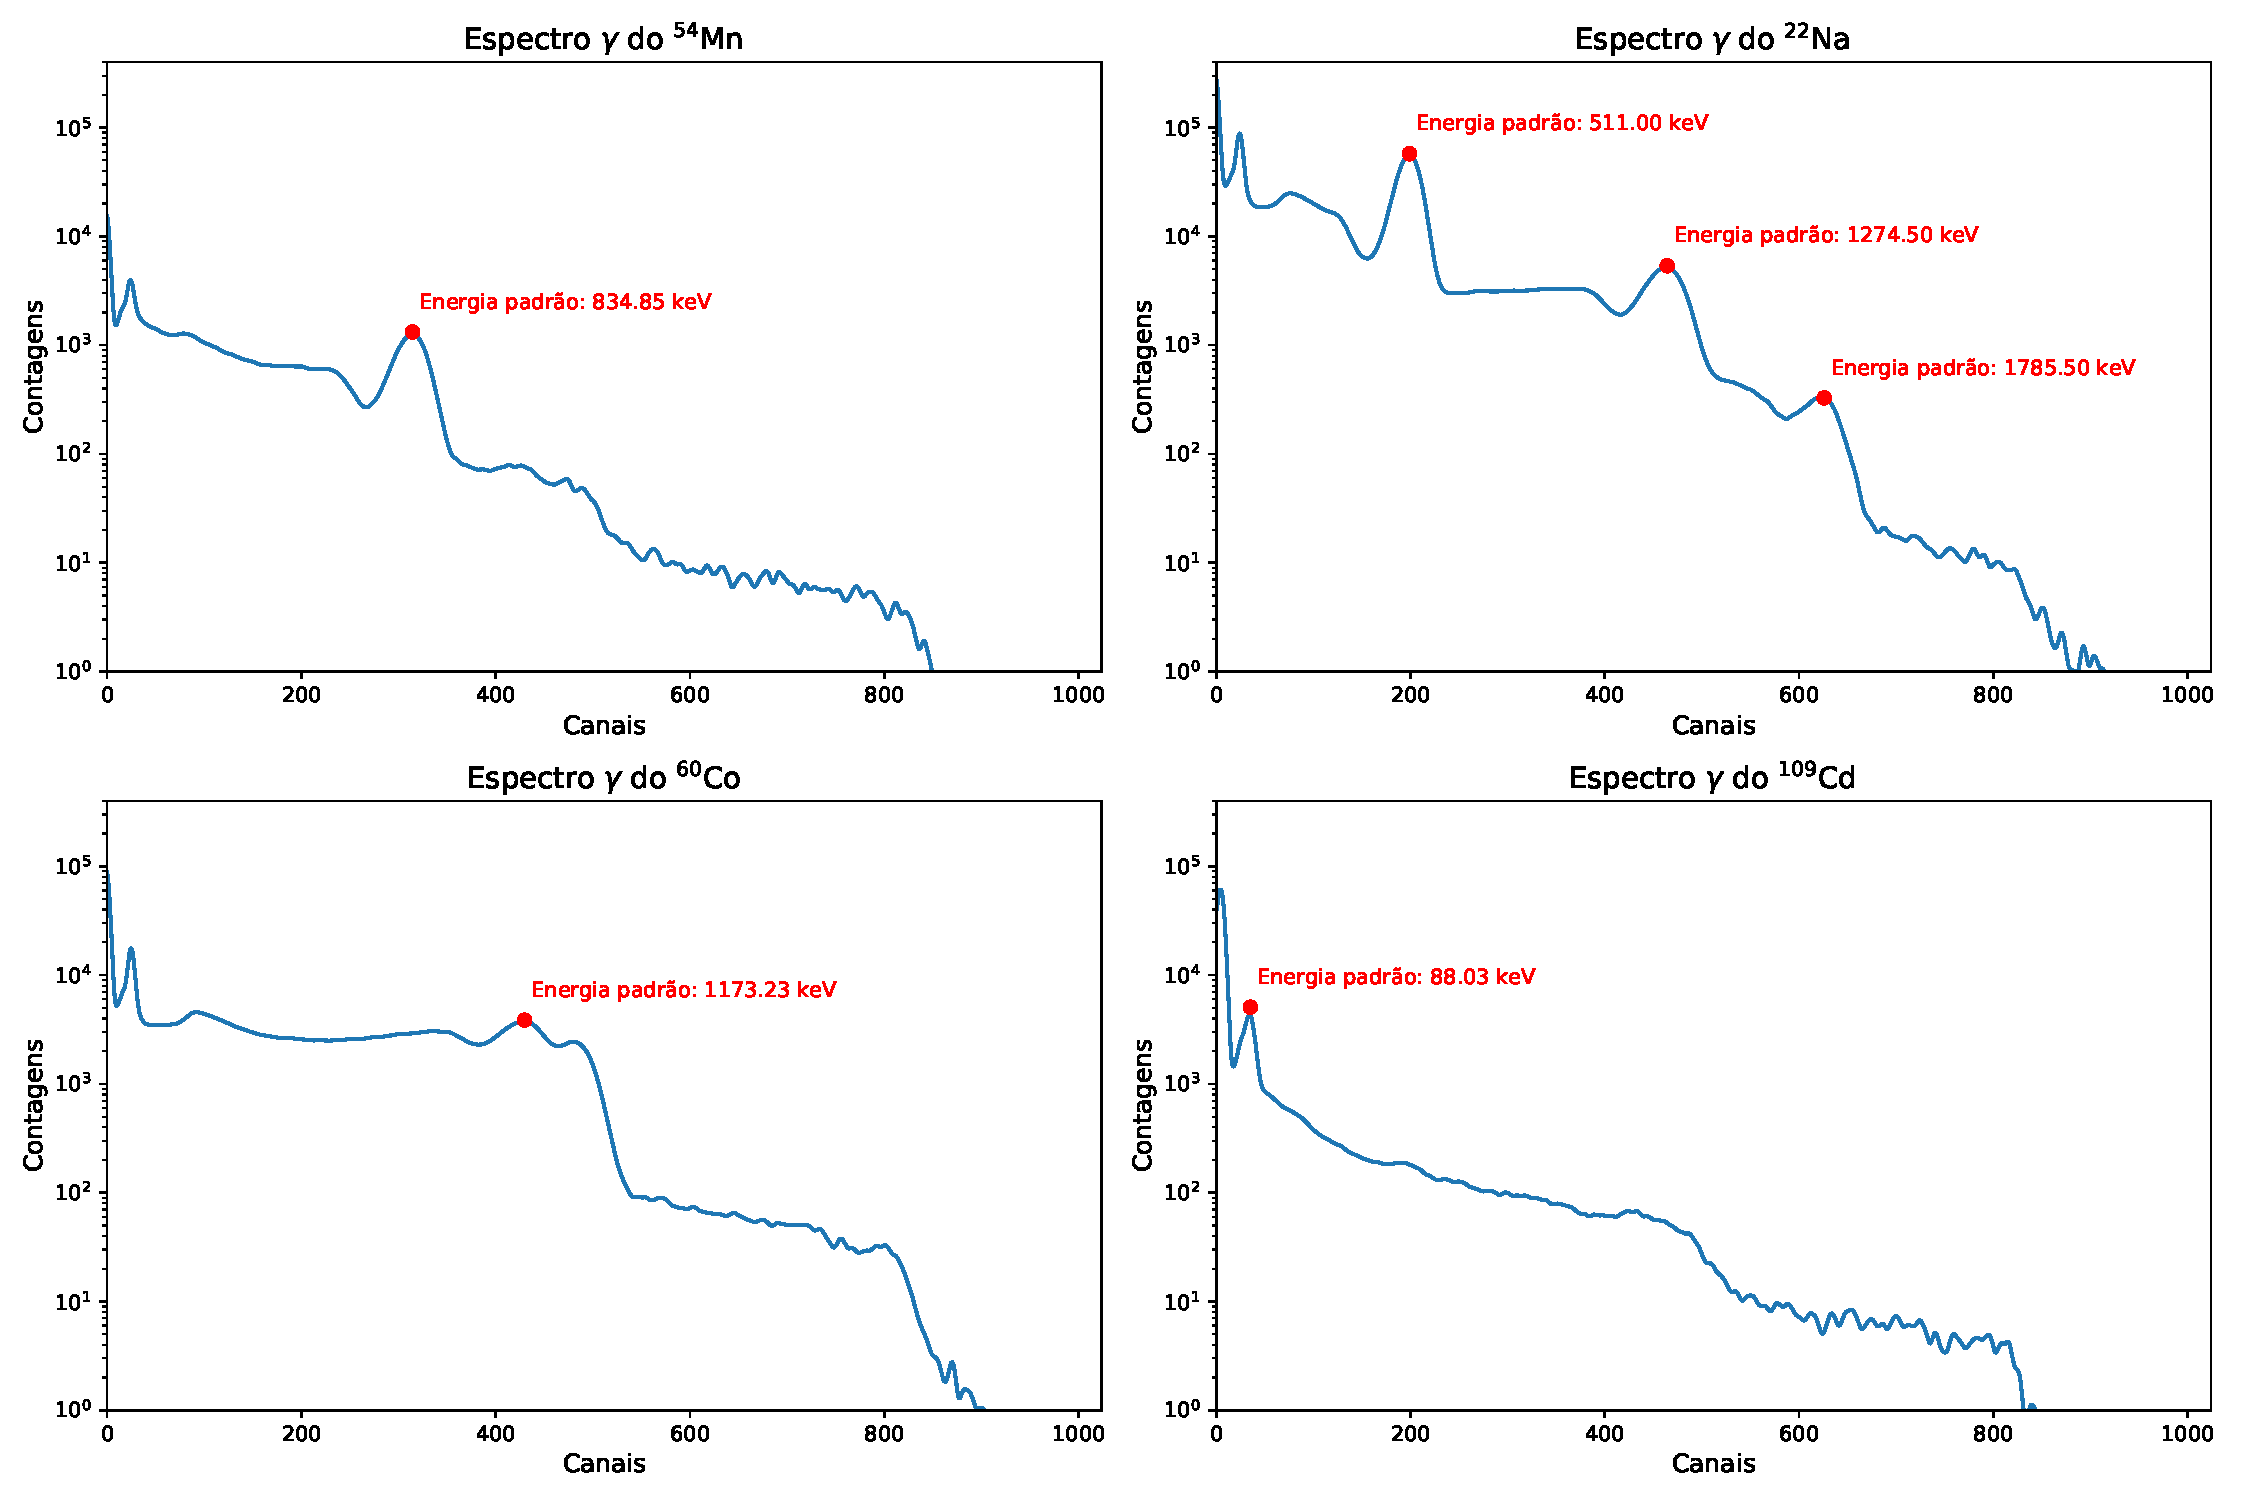
\includegraphics[width=1.00\textwidth]{espectros_amostras_calibracao.pdf}
    \caption{Espectro $\gamma$ das amostras usadas para calibração, juntamente com os picos utilizados para a calibração do espectrômetro.}
    \label{fig:espectro.calibracao}
\end{figure}

\begin{figure}[H]
    \centering
    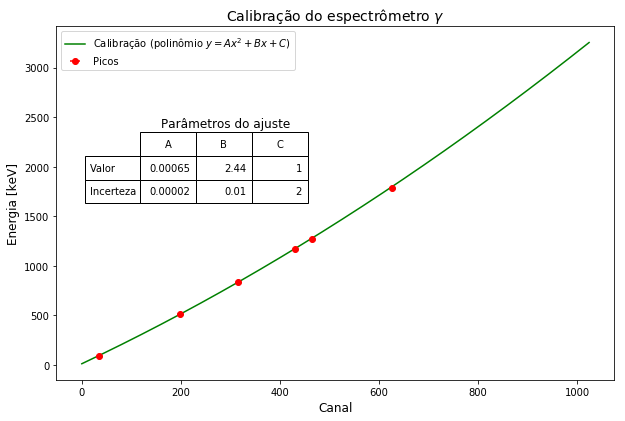
\includegraphics[width=1.00\textwidth]{ajuste_calibracao.png}
    \caption{Calibração do espectrômetro $\gamma$ utilizando um polinômio de grau 2.}
    \label{fig:calibracao}
\end{figure}

Com os valores dos canais do centro de cada linha, juntamente com os valores padrão das energias correspondentes realizamos a calibração do espectrômetro, ajustamos um polinômio de grau 2 da forma

$$ y= Ax^2 + Bx + C $$

\noindent aos dados coletados. Dados, ajustes e parâmetros obtidos, com as incertezas associadas, podem ser vistos na Figura \ref{fig:calibracao}.

\subsection{Espectros das fontes comerciais}

Os espectros tomados das fontes comerciais disponíveis, já calibrados, com picos identificados e comparados com os valores padrão encontrados na literatura \cite{TabRad_v1}-\cite{TabRad_v8} podem ser vistos na Figura \ref{fig:amostras.comerciais}. Observe que os desvios dos valores encontrados para as energias dos fotopicos são inferiores a 10 \%. Observamos também, durante a determinação das incertezas das energias dos picos, que a influência das incertezas na determinação do centróide das linhas é muito inferior à incerteza introduzida pela calibração.

Obtemos também o espectro $\gamma$ de uma amostra desconhecida (cf. Figura \ref{fig:amostra.desconhecida}). A amostra possui duas linhas visíveis: uma corresponde à conhecida linha do ${}^{137}$Cs em 661.66 keV. A outra é próxima à linha de 1120.287 keV do ${}^{214}$Bi, que faz parte da série do ${}^{226}$Ra. Ela com certeza contêm ${}^{137}$Cs, mas provavelmente possui outros isótopos, e não conseguimos conclusivamente identificá-los com o espectro obtido.

\begin{figure}[H]
  \centering
  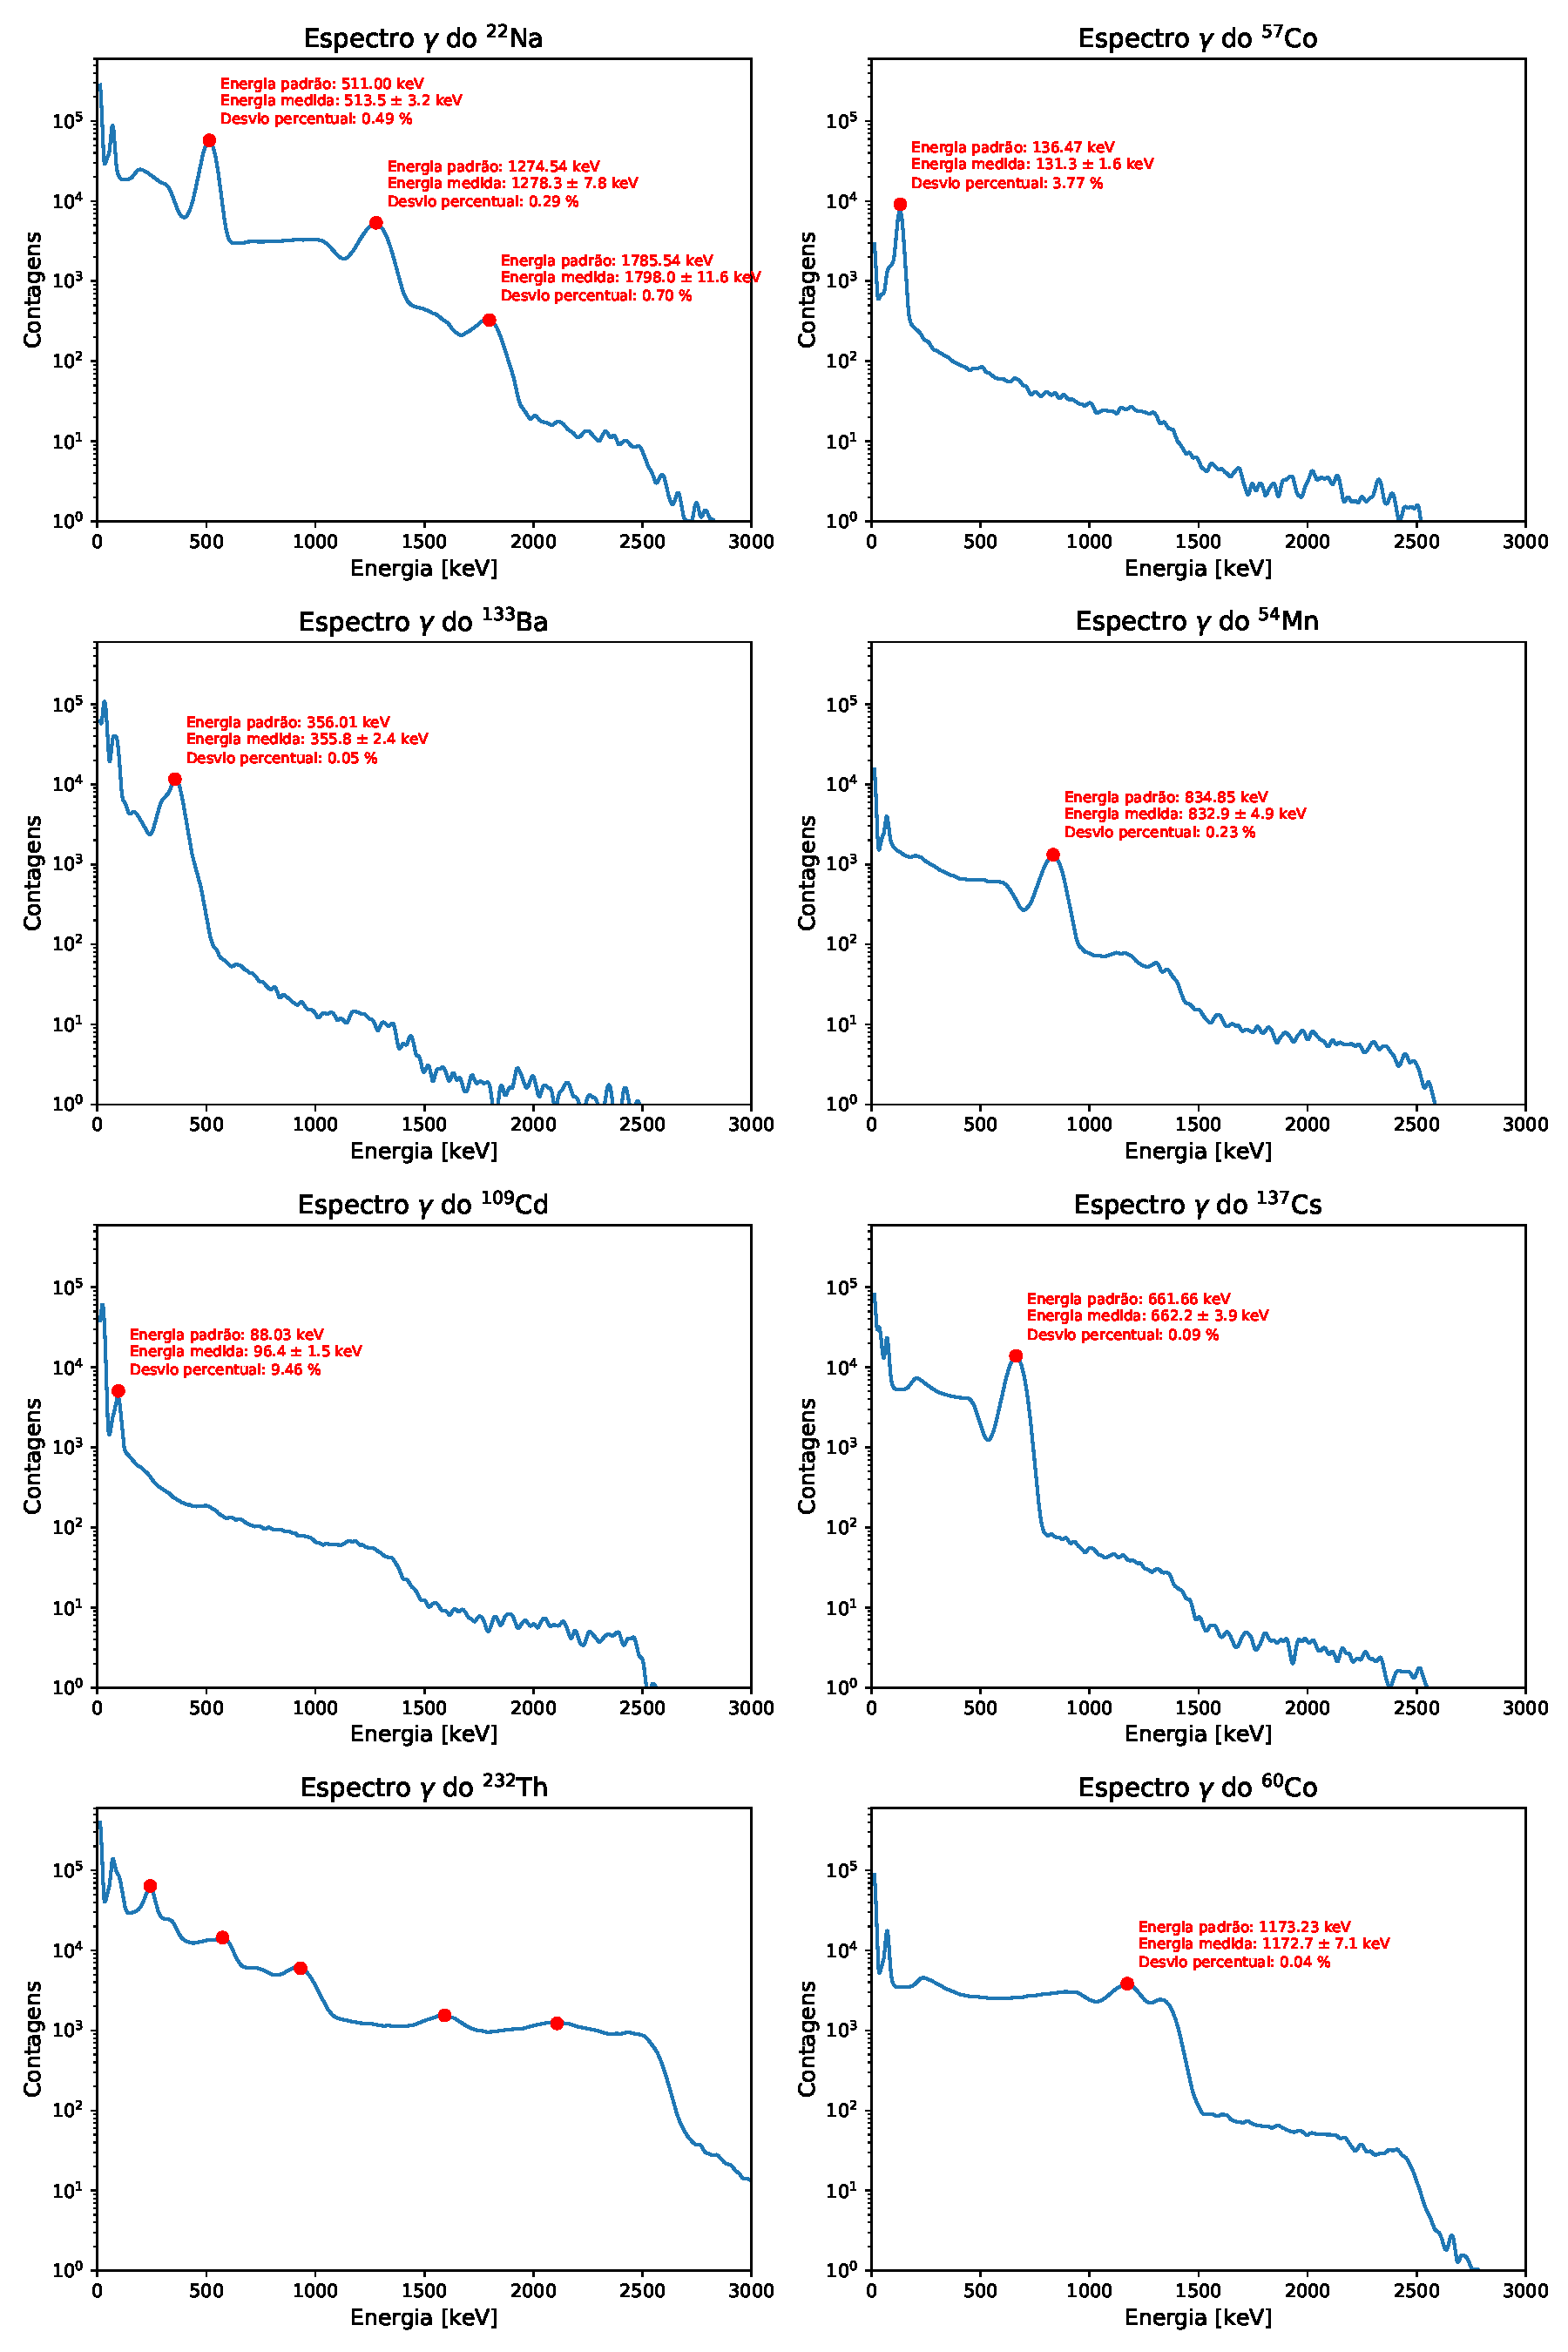
\includegraphics[width=1.00\textwidth]{todos_espectros.pdf}
  \caption{Espectros das fontes comerciais.}
  \label{fig:amostras.comerciais}
\end{figure}

\begin{figure}[H]
  \centering
  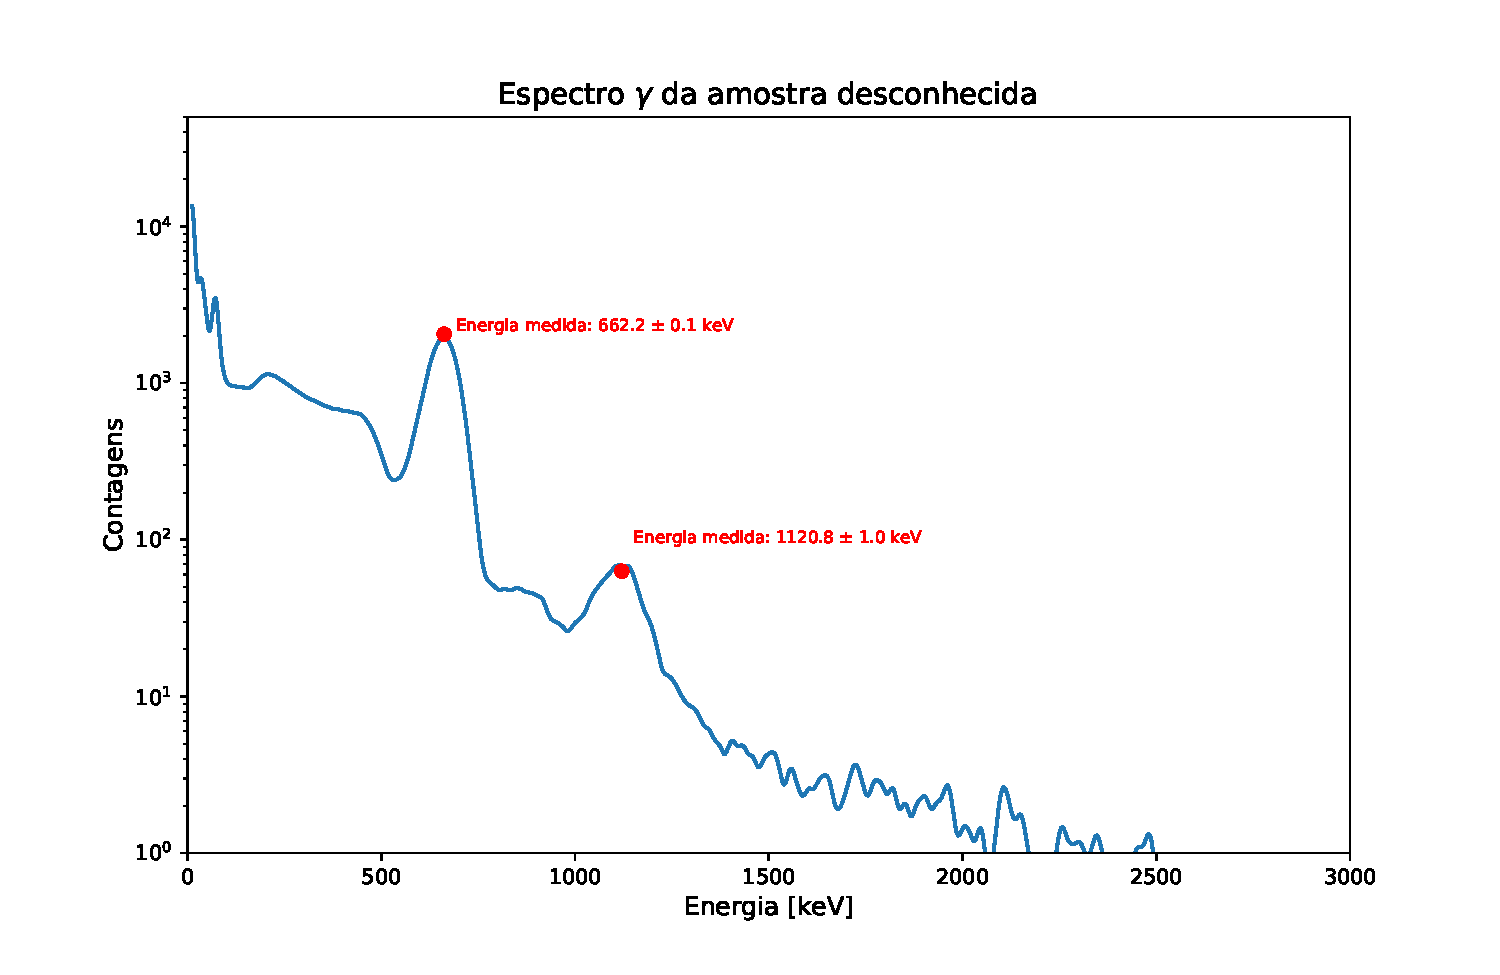
\includegraphics[width=0.95\textwidth]{amostra_desconhecida.pdf}
  \caption{Espectros de amostra desconhecida.}
  \label{fig:amostra.desconhecida}
\end{figure}

\subsection{Verificação da calibração}

Como verificação da calibração medimos o espectro de uma fonte de ${}^{137}$Cs, obtendo pelo procedimento descrito anteriormente a energia do pico, com sua respectiva incerteza obtida propagando as incertezas conhecidas para os parâmetros da calibração e para o valor do centro da linha (cf. Figura \ref{fig:verificacao.calibracao}). Comparação com o valor de referência desta linha mostra um desvio de apenas $0.1$ \%.

\begin{figure}[H]
  \centering
  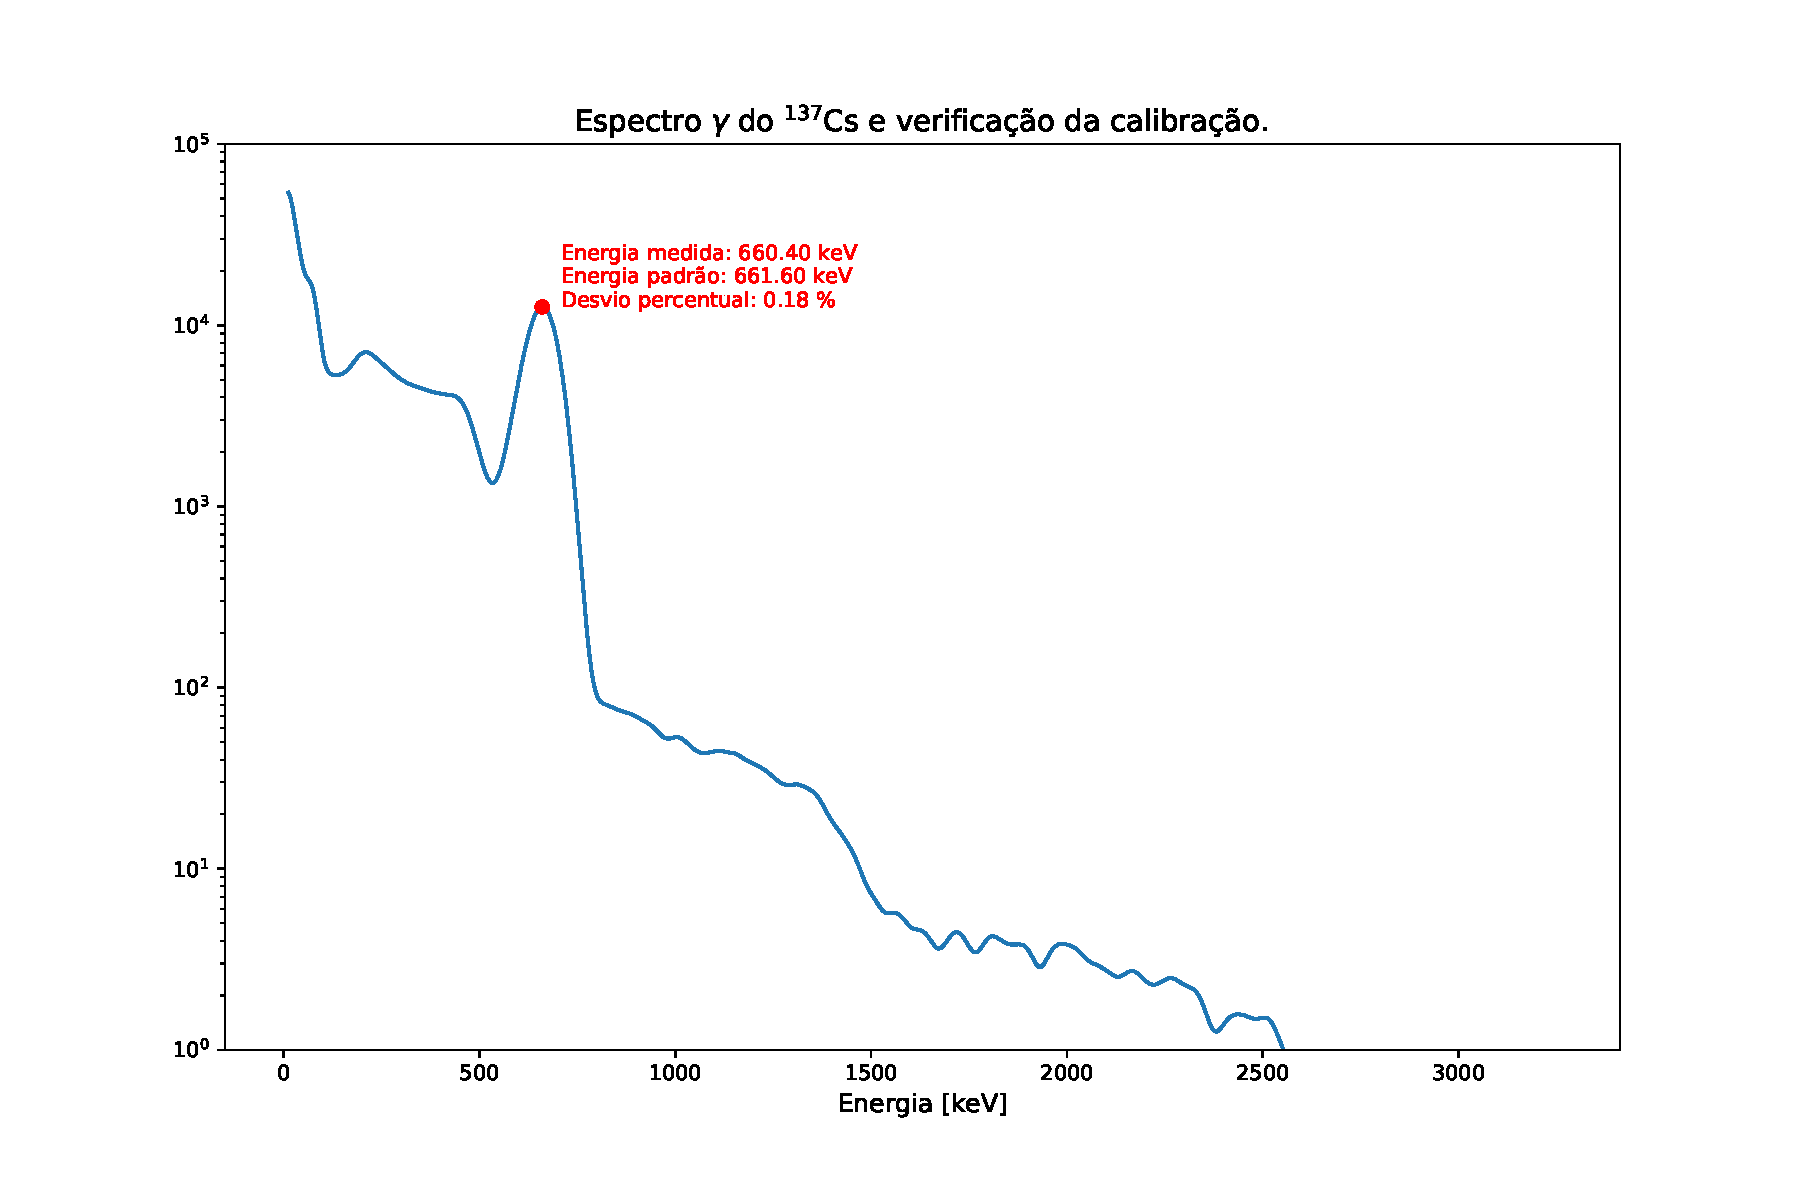
\includegraphics[width=0.93\textwidth]{verificacao_calibracao.pdf}
  \caption{Espectro $\gamma$ do ${}^{137}$Cs, utilizado para verificação da calibração realizada.}
  \label{fig:verificacao.calibracao}
\end{figure}

\subsection{Resolução em energia}

O gráfico da dependência na energia da resolução relativa do espectrômetro encontra-se na Figura \ref{fig:resolucao.loglog}.

\begin{figure}[h]
  \centering
  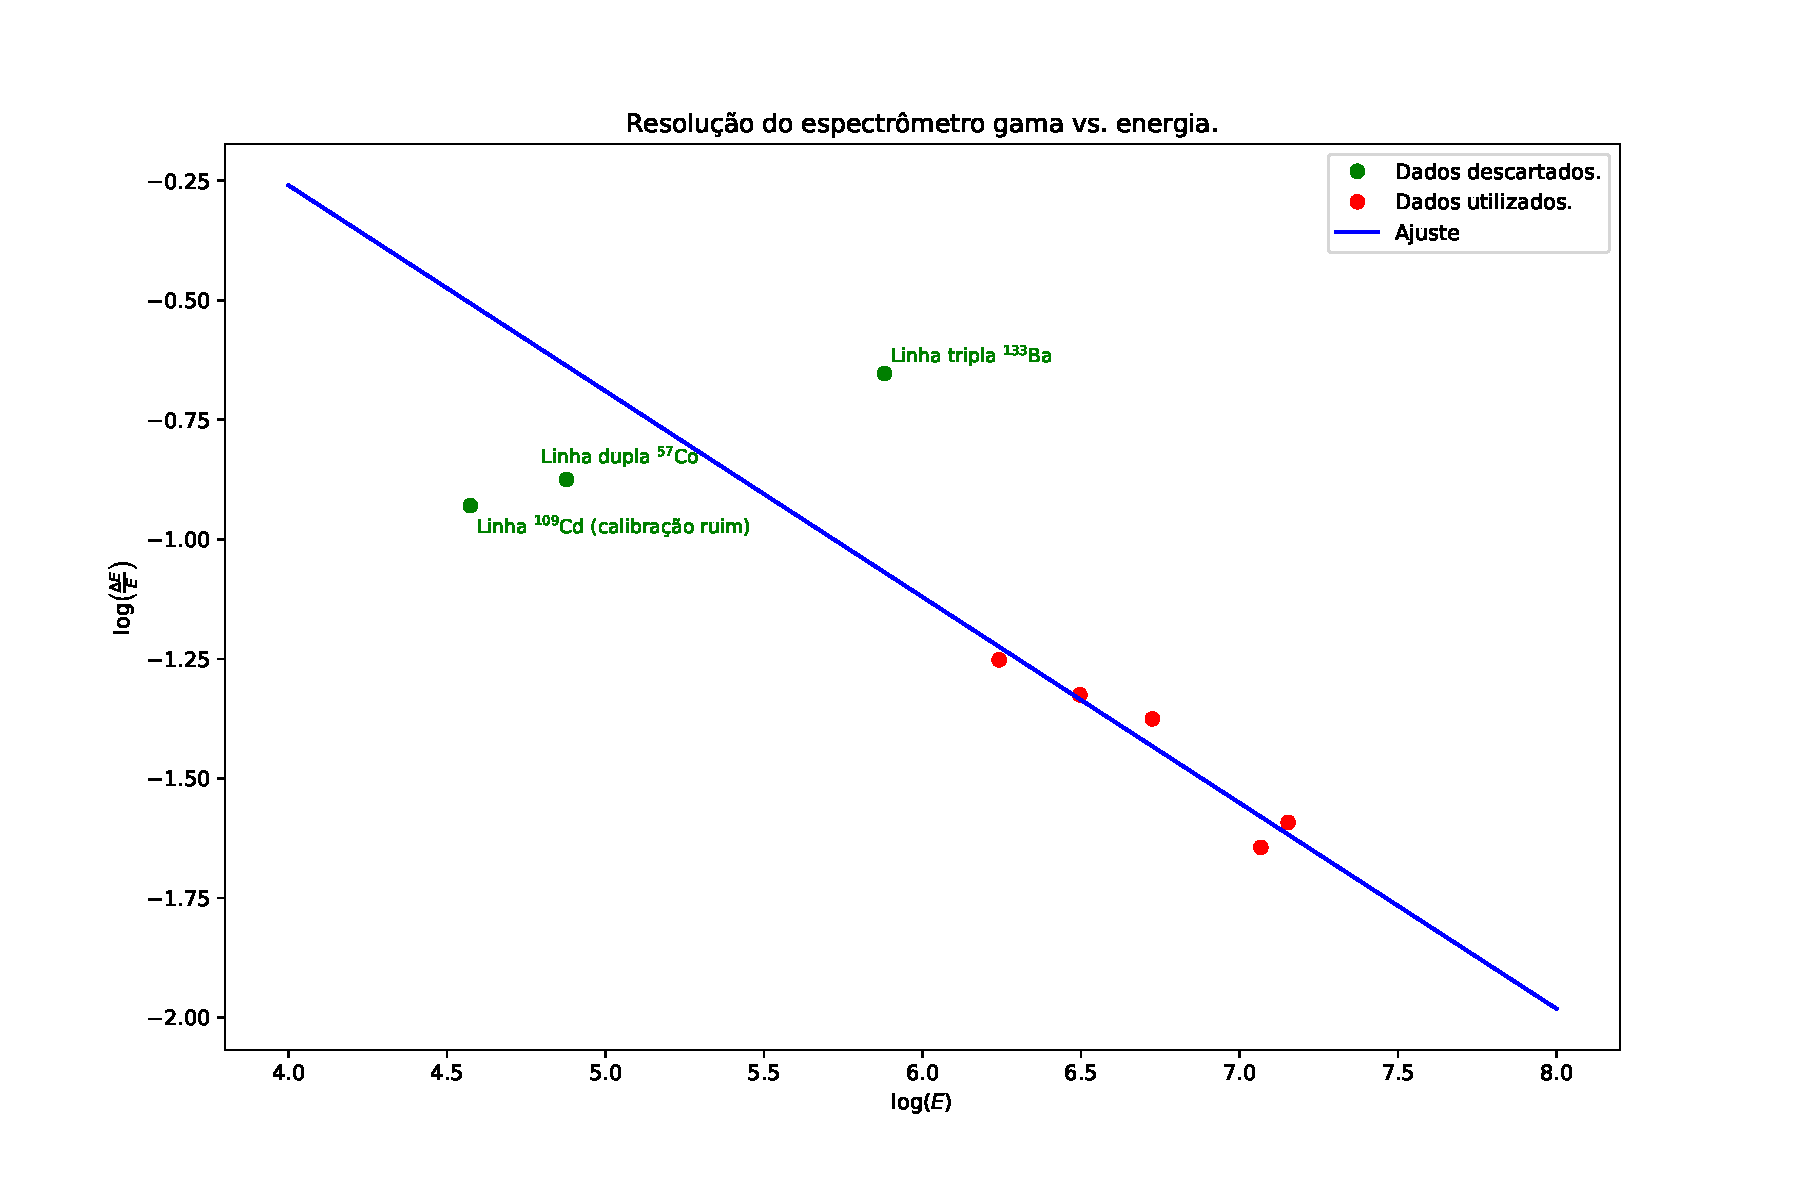
\includegraphics[width=1.00\textwidth]{resolucao_loglog.pdf}
  \caption{Resolução do espectrômetro gama vs. energia, em escala logaritmica.}
  \label{fig:resolucao.loglog}
\end{figure}

Note que a reta ajusta relativamente bem os dados obtidos. O valor obtido para o coeficiente angular, $-0.43 \pm 0.07$ está de acordo com o valor teórico esperado ($-0.5$). Três pontos diferem consideravelmente dos demais. Um deles é uma linha múltipla do ${}^{133}$Ba que nosso espectrômetro foi incapaz de separar: na região entre 200 e 400 keV há três linhas espectrais, em $302.8508$, $356.0129$ e $383.8485$ keV (de fato podemos ver em nosso espectro uma assimetria da linha, indicativa de artefatos não resolvidos no espectro - cf. Figura \ref{fig:linha.tripla}). 

\begin{figure}[H]
  \centering
  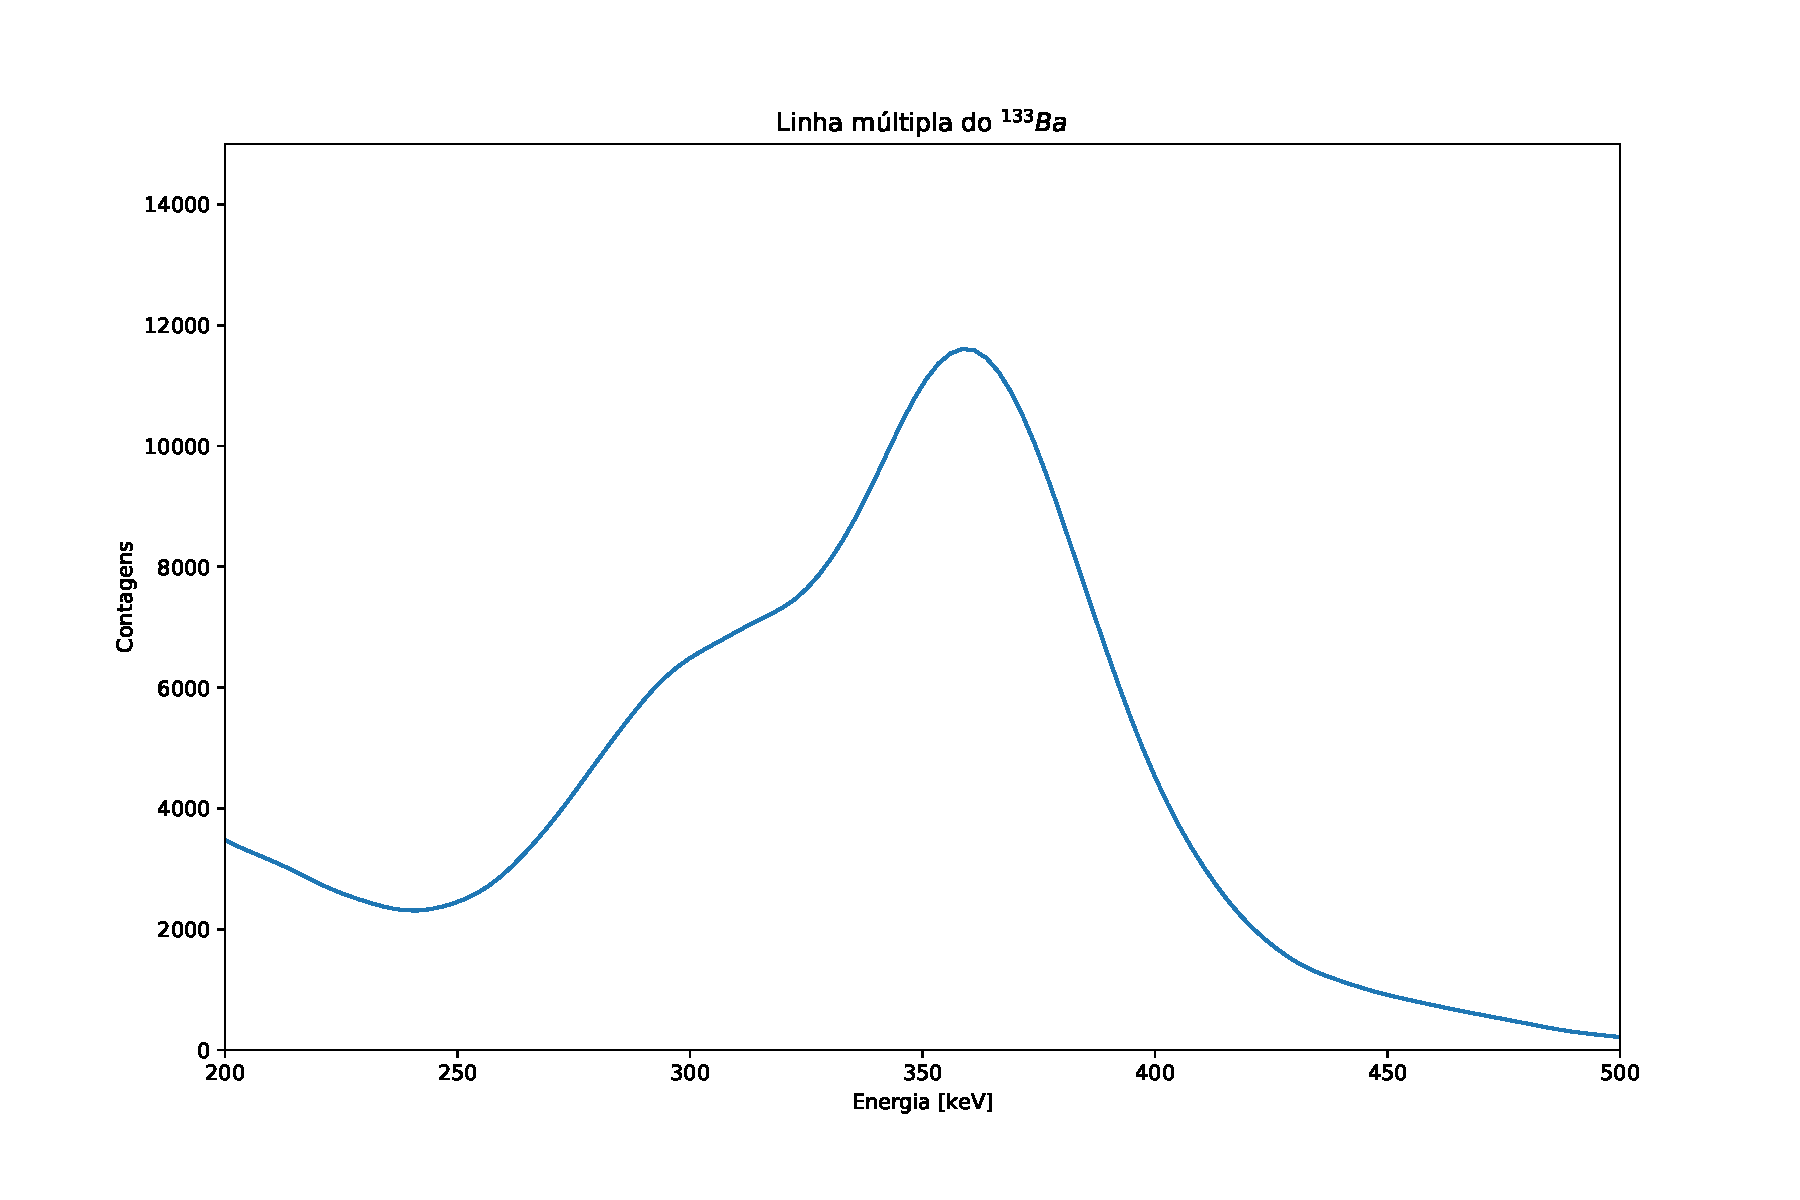
\includegraphics[width=0.71\textwidth]{linhatripla.pdf}
  \caption{Linha tripla não resolvida do ${}^{133}$Ba.}
  \label{fig:linha.tripla}
\end{figure}

Outro é uma linha múltipla do ${}^{57}$Co e por fim temos a linha do ${}^{109}$Cd, que já está em uma região onde a calibração é bastante ruim (verificamos anteriormente que a calibração produz desvios da ordem de 10 \% nesta região de baixas energias). Estes pontos não foram utilizados para o ajuste linear.

Fizemos também o gráfico de $\left(\frac{\Delta E}{E}\right)^2$ vs. $\frac{1}{E}$ (veja Figura \ref{fig:resolucao.lin}). Novamente, os dados das linhas do ${}^{133}$Ba, ${}^{57}$Co e ${}^{109}$Cd distoam dos demais. O ajuste é entretanto bom, com coeficiente angular de $38 \pm 6$ keV e coeficiente linear de $0.011 \pm 0.008$.

\begin{figure}[H]
  \centering
  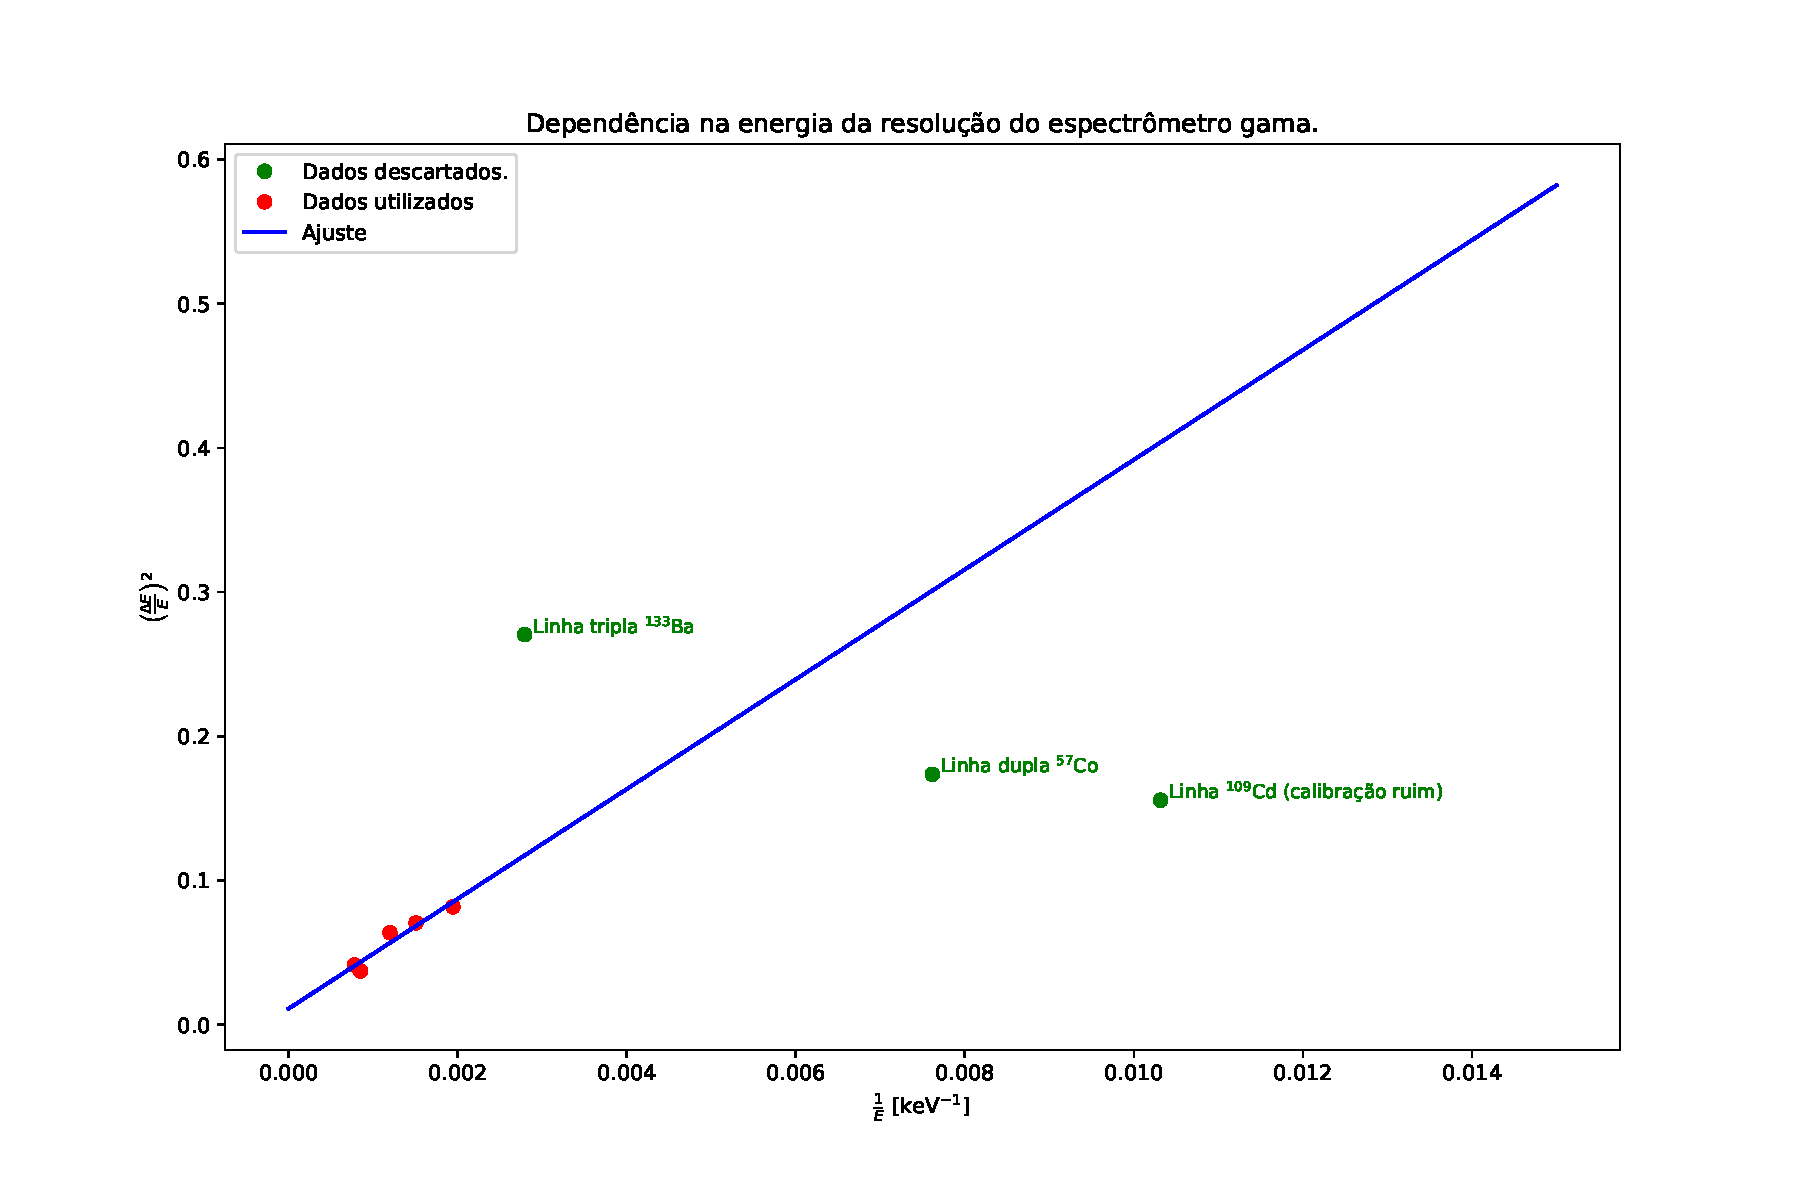
\includegraphics[width=1.0\textwidth]{resolucao_lin.pdf}
  \caption{Resolução quadrática relativa do espectrômetro gama vs. inverso da energia.}
  \label{fig:resolucao.lin}
\end{figure}

\subsection{Espalhamento Compton}

Os espectros coletados das fontes de ${}^{22}$Na, ${}^{137}$Cs e ${}^{54}$Mn, evidenciando o espalhamento Compton, estão plotados na Figura \ref{fig:espectros.compton}. Tanto o pico de Backscattering quando o Compton Edge são facilmente visíveis.

\begin{figure}[H]
\centering
  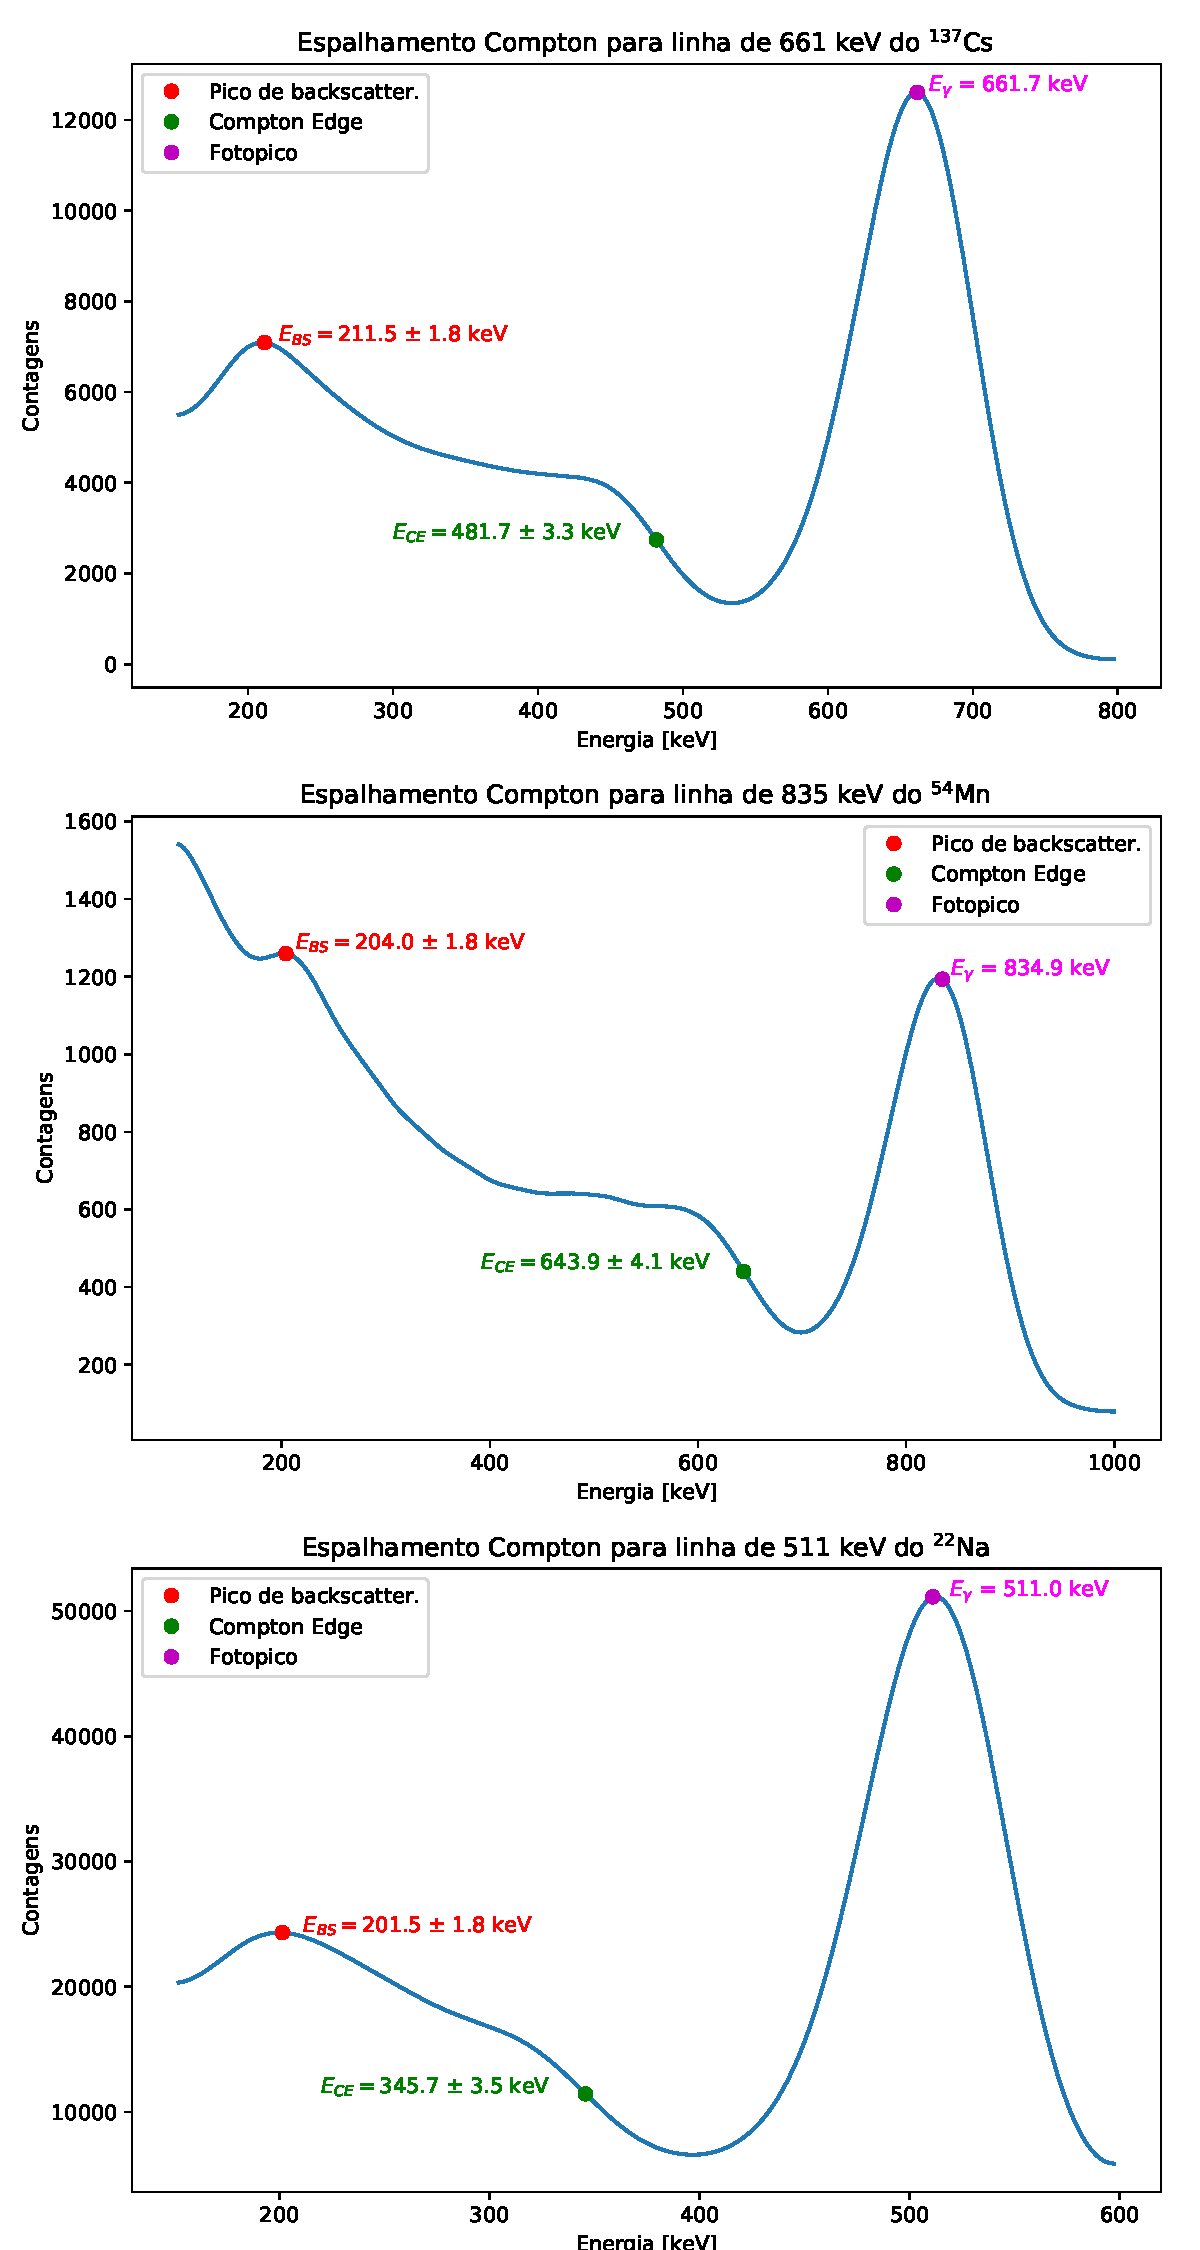
\includegraphics[width=0.8\textwidth]{plots_compton}
  \caption{Espectros $\gamma$ de amostras de ${}^{22}$Na, ${}^{137}$Cs e ${}^{54}$Mn exibindo o pico de Backscattering e o Compton Edge característicos do espalhamento Compton.}
  \label{fig:espectros.compton}
\end{figure}

Conforme descrito na Metodologia, medimos, usando as energias encontradas para o Compton Edge e para o pico de Backscattering, a massa do elétron e sua incerteza. Estas 6 medições de massa estão ilustradas na Figura \ref{fig:dispersao.massas} (as barras de erros correspondem a 1 desvio padrão). Calculamos a médias ponderada destas medidas, obtendo

$$ m_e = 512 \pm 2 \text{ keV/c$^2$} $$

\noindent valor que concorda com o valor recomendado pelo CODATA \cite{codata2014}, de 

$$ m_e = 510.9989461(31) \text{ keV/c$^2$} $$

Calculando o $\chi^2$ normalizado pelo número de gaus de liberdade, porém, obtemos o valor de

$$ \chi^2 = 108.54 $$

Este valor é \textbf{muito} alto, dado que o valor esperado é de cerca de 1. De fato, analisando o gráfico da dispersão dos valores usados para compor a média (cf. Figura \ref{fig:dispersao.massas}) vemos que a maior parte dos massas medidas está vários desvios padrões distante da média obtida. É provável que algum erro sistemático esteja afetando as medidas. As medidas obtidas a partir da energia do pico de backscattering são, por exemplo, todas vários desvios padrões maiores que a média, enquanto as medidas a partir do Compton Edge são consideravelmente inferiores à média. 

Uma possibilidade importante de erro sistemático é o fato de uma quantidade apreciável de fótons retroespalhados a ângulos ligeiramente menores que 180$^\circ$ adentrarem o detector e depositarem sua energia no mesmo. Estes fótons possuem energia maior que a energia dos fótons espalhados frontalmente, e portanto tendem a aumentar a energia medida para o pico de backscattering $E_{BS}$. Na equação \eqref{eq:massaeletron.bs} vemos, porém, que um aumento em $E_{BS}$ gera um aumento na massa medida para o elétron, o que explica os resultados obtidos. Note ainda que conforme a energia do fotopico aumenta este efeito torna-se menor, o que novamente é consistente com o observado (cf. a Figura \ref{fig:dispersao.massas}, notando que as energias dos fotopicos são, $511.0$ keV, $661.7$ keV e $934.9$ keV para o ${}^{22}$Na, ${}^{137}$Cs e ${}^{54}$Mn, respectivamente).

\begin{figure}[H]
  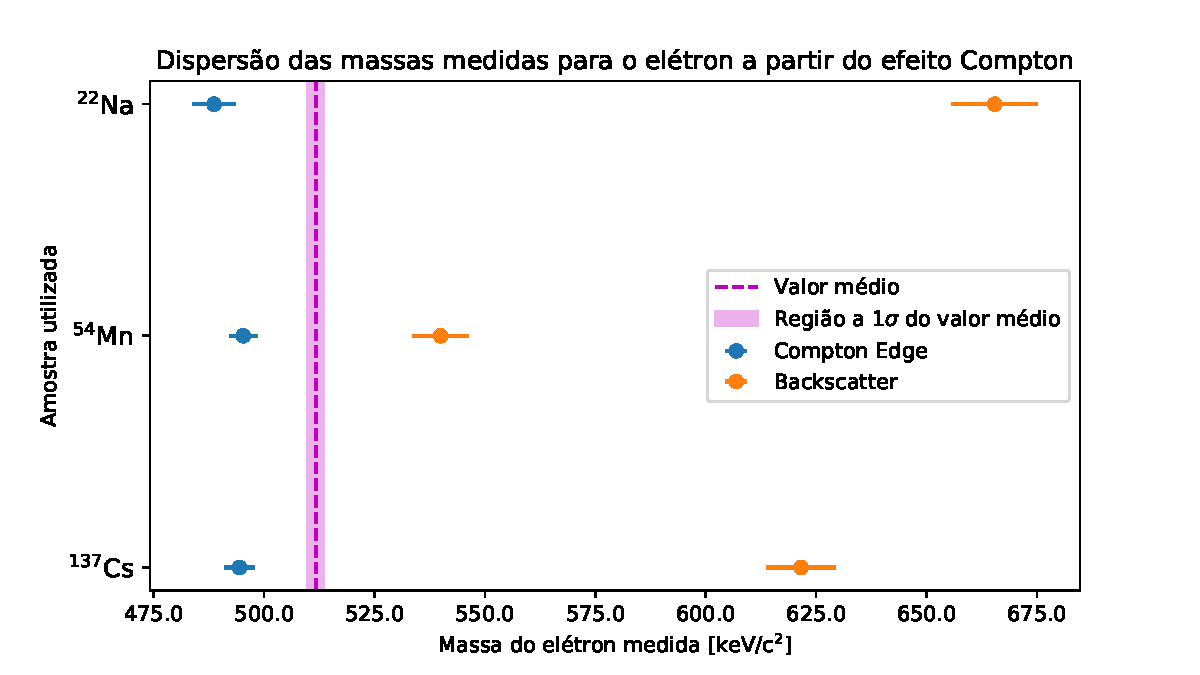
\includegraphics[width=0.9\textwidth]{dispersao_massas}
  \caption{Valores medidos para a massa do elétron, segundo amostra e forma de medição.}
  \label{fig:dispersao.massas}
\end{figure}

\subsection{Produção e aniquilação de pares}

A produção de pares foi observada no espectro $\gamma$ do ${}^{22}$Na (cf. Figura \ref{fig:espectro.na}). Note a presença do pico com energia de $513.5$ keV, próxima de $511$ keV. Este pico é devido à aniquilação dos pósitrons emitidos pela amostra com elétrons do meio ao redor, sendo apenas um dos fótons produzidos coletados pelo detector pois ambos saem quase diametralmente opostos no referencial do laboratório. 

Observamos também uma transição $\gamma$ do ${}^{22}$Na e um pico de soma das duas linhas, que ocorre pela incapacidade do detector de separar dois fótons que chegam no sistema praticamente ao mesmo tempo.

\begin{figure}[H]
  \centering
  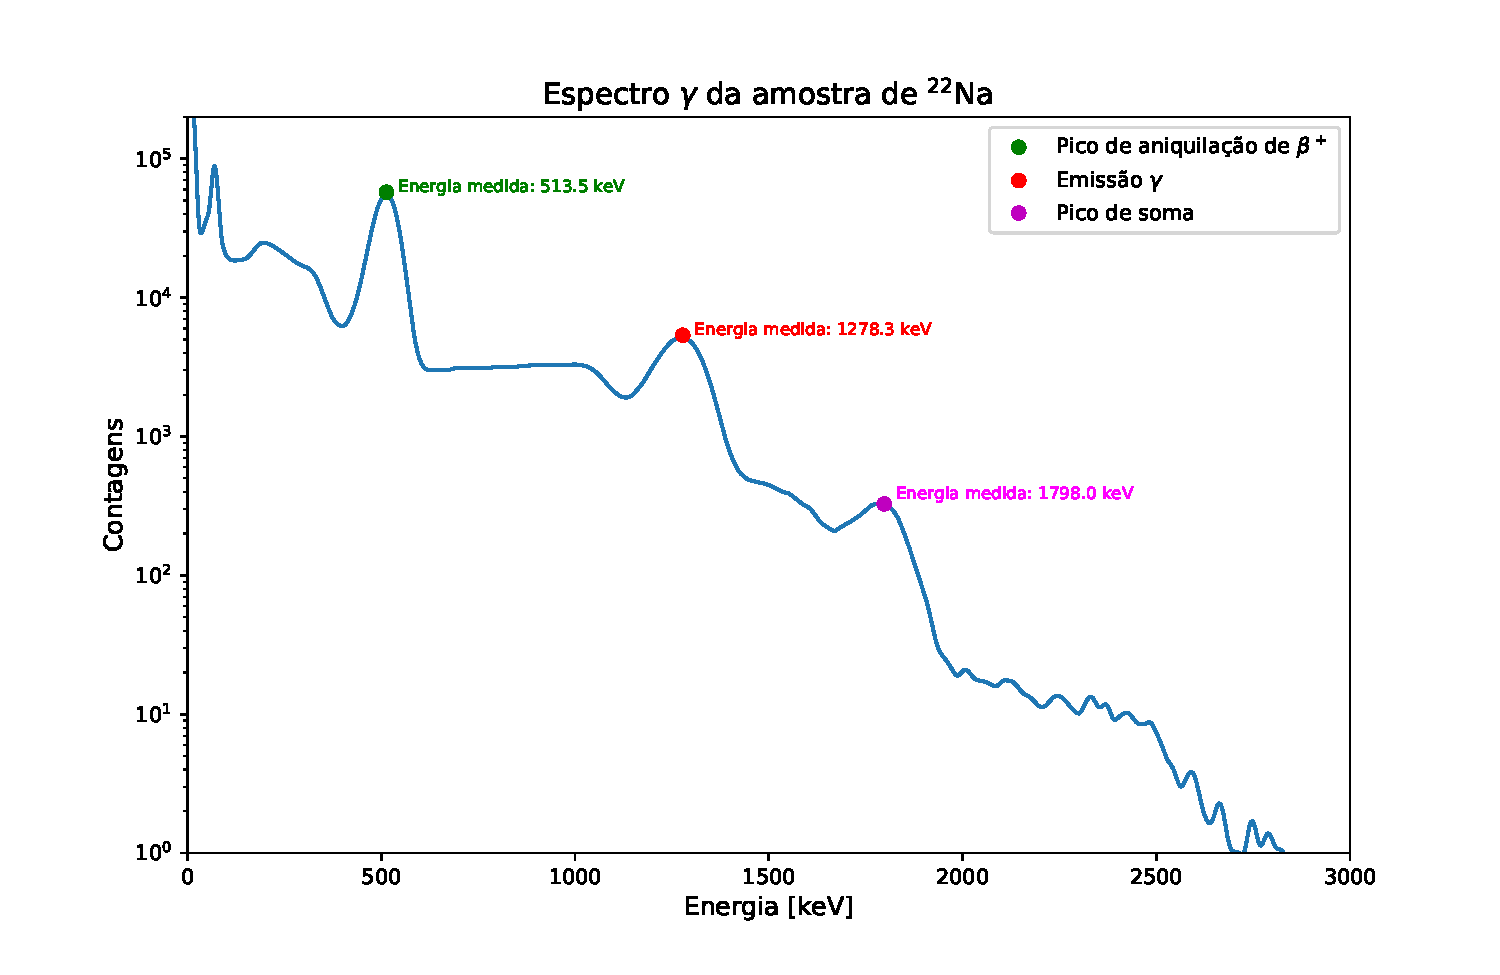
\includegraphics[width=0.9\textwidth]{na22}
  \caption{Espectro do ${}^{22}$Na, exibindo fótons provinientes da aniquilação de pósitrons.}
  \label{fig:espectro.na}
\end{figure}

Não conseguimos observar a produção de pares no espectro do ${}^{232}$Th, tanto pelo ruído e pela presença de vários artefatos no espectro em altas energias como por nossa calibração não funcionar bem nesta região.

\subsection{Absorção de raios gama}

Com os dados obtidos e a análise realizada conforme descrito na Metodologia obtemos o gráfico da Figura \ref{fig:absorcao.gamma}.

\begin{figure}[H]
  \centering
  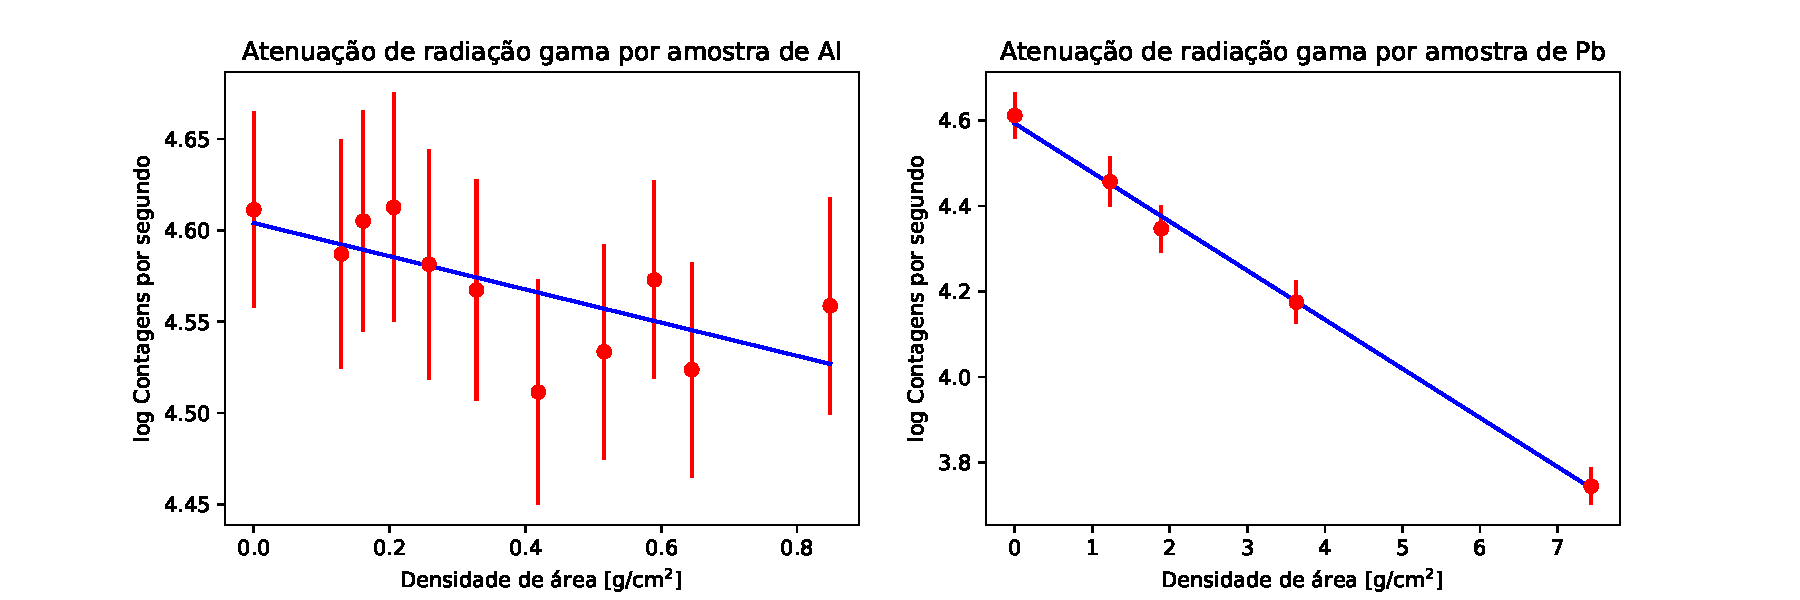
\includegraphics[width=1.0\textwidth]{absorcao_gamma.pdf}
  \caption{Absorção de radiação $\gamma$ por amostras de Alumínio e Chumbo.}
  \label{fig:absorcao.gamma}
\end{figure}

Denotando por $a$ e $b$ os coeficientes angular e linear, respectivamente, dos ajustes lineares realizados, encontramos para as amostras de Alumínio

\begin{align*}
a_{Al} &= -0.09 \pm 0.03 \text{ cm}^2\text{/g} \\
b_{Al} &= 4.60 \pm 0.02
\end{align*}

\noindent e para as amostras de Chumbo

\begin{align*}
a_{Pb} &= -0.115 \pm 0.03 \text{ cm}^2\text{/g} \\
b_{Pb} &= 4.59 \pm 0.01
\end{align*}

Note que os coeficientes lineares do ajustes para o Pb e o Al são consistentes (como deveriam ser, pois correspondem à taxa de contagens na ausência de obstáculos). Para o Alumínio, o coeficiente angular do ajuste nos fornece um coeficiente de atenuação de 

\[
\left(\frac{\mu}{\rho}\right)_{Al} = 0.09 \pm 0.03\text{ cm}^2\text{/g}
\]

\noindent valor consistente com o valor padrão do NIST\cite{nist_absorption} para o coeficiente de atenuação a uma energia de $600$ keV (0.0780 cm$^2$/g).

Já para o Chumbo, o coeficiente obtido foi

\[
\left(\frac{\mu}{\rho}\right)_{Pb} = 0.115 \pm 0.003\text{ cm}^2\text{/g}
\]

\noindent próximo do valor padrão do NIST\cite{nist_absorption} para o coeficiente de atenuação a uma energia de $600$ keV (0.1248 cm$^2$/g). A inconsistência pode ser devida tanto ao fato de o valor padrão ser dada numa energia diferente da utilizada quanto pois na verdade não medimos apenas a radiação que atravessou o material sem sofrer espalhamento, mas uma pequena parcela da radiação espalhada também. Com isto a taxa de contagens obtida experimentalmente é ligeiramente superestimada, o que pode fazer com que o coeficiente angular do ajuste seja subestimado.

\subsection{Estatísticas de contagem}

A partir dos dados obtidos e dos valores calculados para as médias e desvios padrões das distribuições poissonianas destes dados, plotamos os histogramas da Figura \ref{fig:estatisticas.contagem}. Note que, visualmente, o modelo teórico ajusta muito bem os dados obtidos. Observe ainda que, quanto maior o tempo de aquisição, menor é o desvio padrão das medidas. Isto concorda tanto com o senso comum, de que as médias ficam mais definidas para um maior número de medidas, quanto com a expressão obtida anteriormente para a variância da taxa de contagens.

\begin{figure}[h]
  \centering
  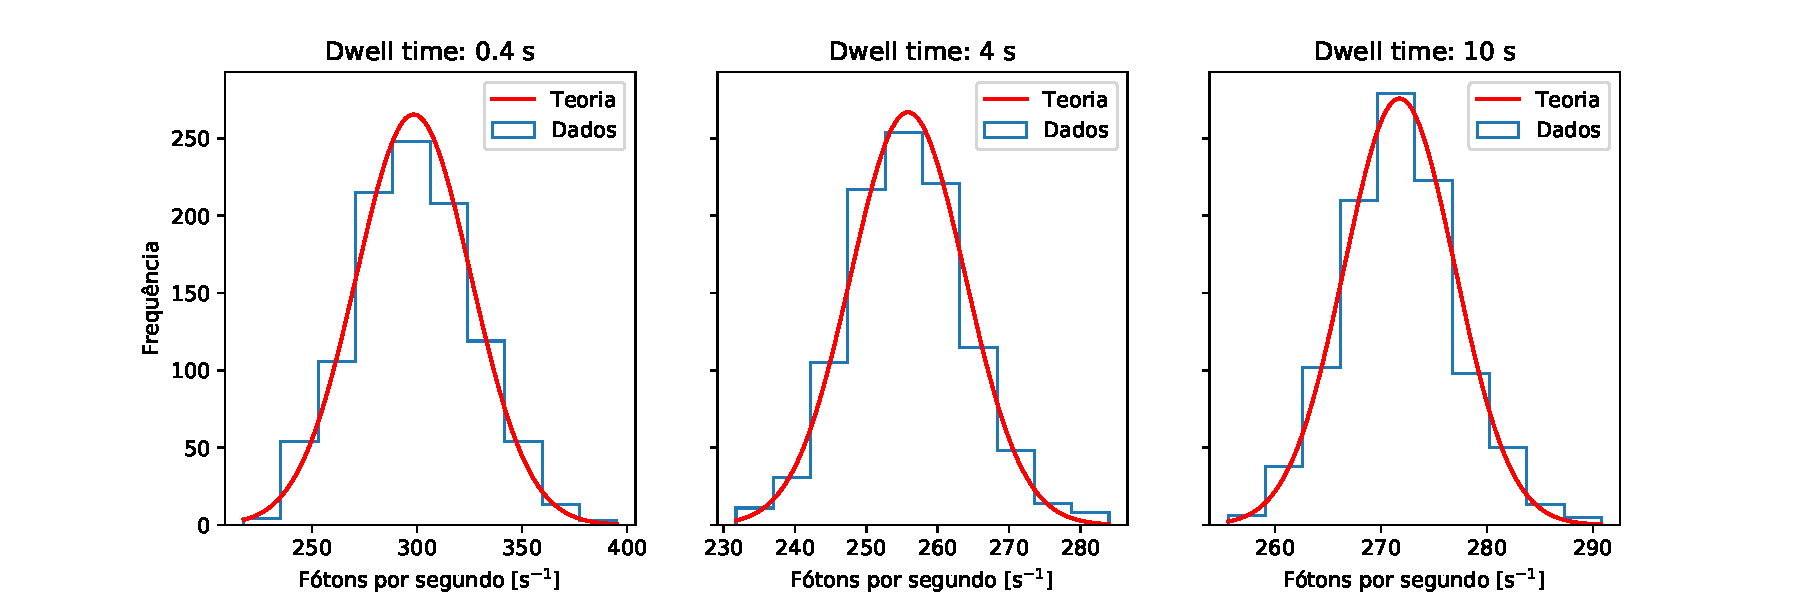
\includegraphics[width=1.0\textwidth]{estatisticas.pdf}
  \caption{Estatísticas de contagem.}
  \label{fig:estatisticas.contagem}
\end{figure}

\subsection{Camisa de Tório}

Os espectros obtidos para a exposição de 24 h da manta de Tório e  da radiação de fundo (background) foram plotados na Figura \ref{fig:espectro.manta.bkg}. Note que eles são bastante semelhantes: a radiação de fundo é principalmente devida ao Tório presente no solo e nas paredes do edifício do laboratório.

\begin{figure}[H]
  \centering
  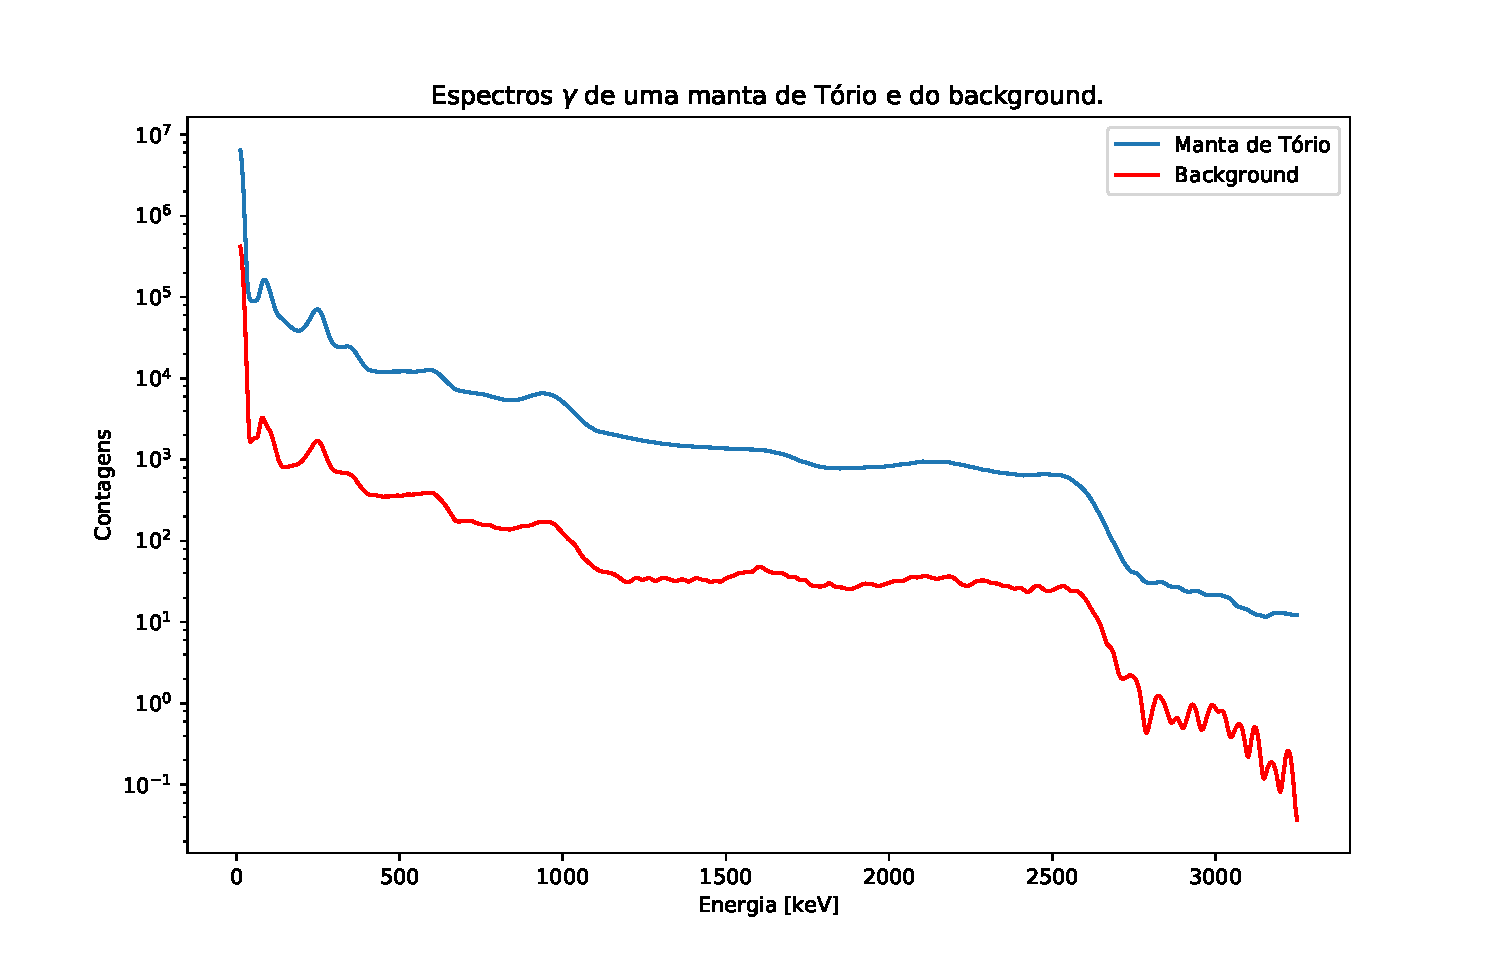
\includegraphics[width=0.9\textwidth]{espectros_manta_bkg}
  \caption{Espectros $\gamma$ para exposições de 24 h de uma manta de Tório e da radiação de fundo.}
  \label{fig:espectro.manta.bkg}
\end{figure}

Procedemos então à obtenção da razão entre as atividades do ${}^{228}$Ra e do ${}^{228}$Th. Procedendo como descrito na seção \ref{sec:metodologia.torio}, ajustamos a função \eqref{eq:tres.picos} aos dados obtidos, obtendo para as amplitudes e médias das gaussianas

\begin{align*}
  A_1 &= 2.11552705(2)  \\
  A_2 &= 1.3(3) \cdot 10^5 \\
  A_3 &= 1.8(3) \cdot 10^5
\end{align*}

\begin{align*}
  E_1 &= 861.9 \text{ keV} \\
  E_2 &= 921(4) \text{keV} \\
  E_3 &= 978(5) \text{keV}
\end{align*}

O gráfico do ajuste obtido pode ser visto na Figura \ref{fig:atividade.ac}.

\begin{figure}[H]
  \centering
  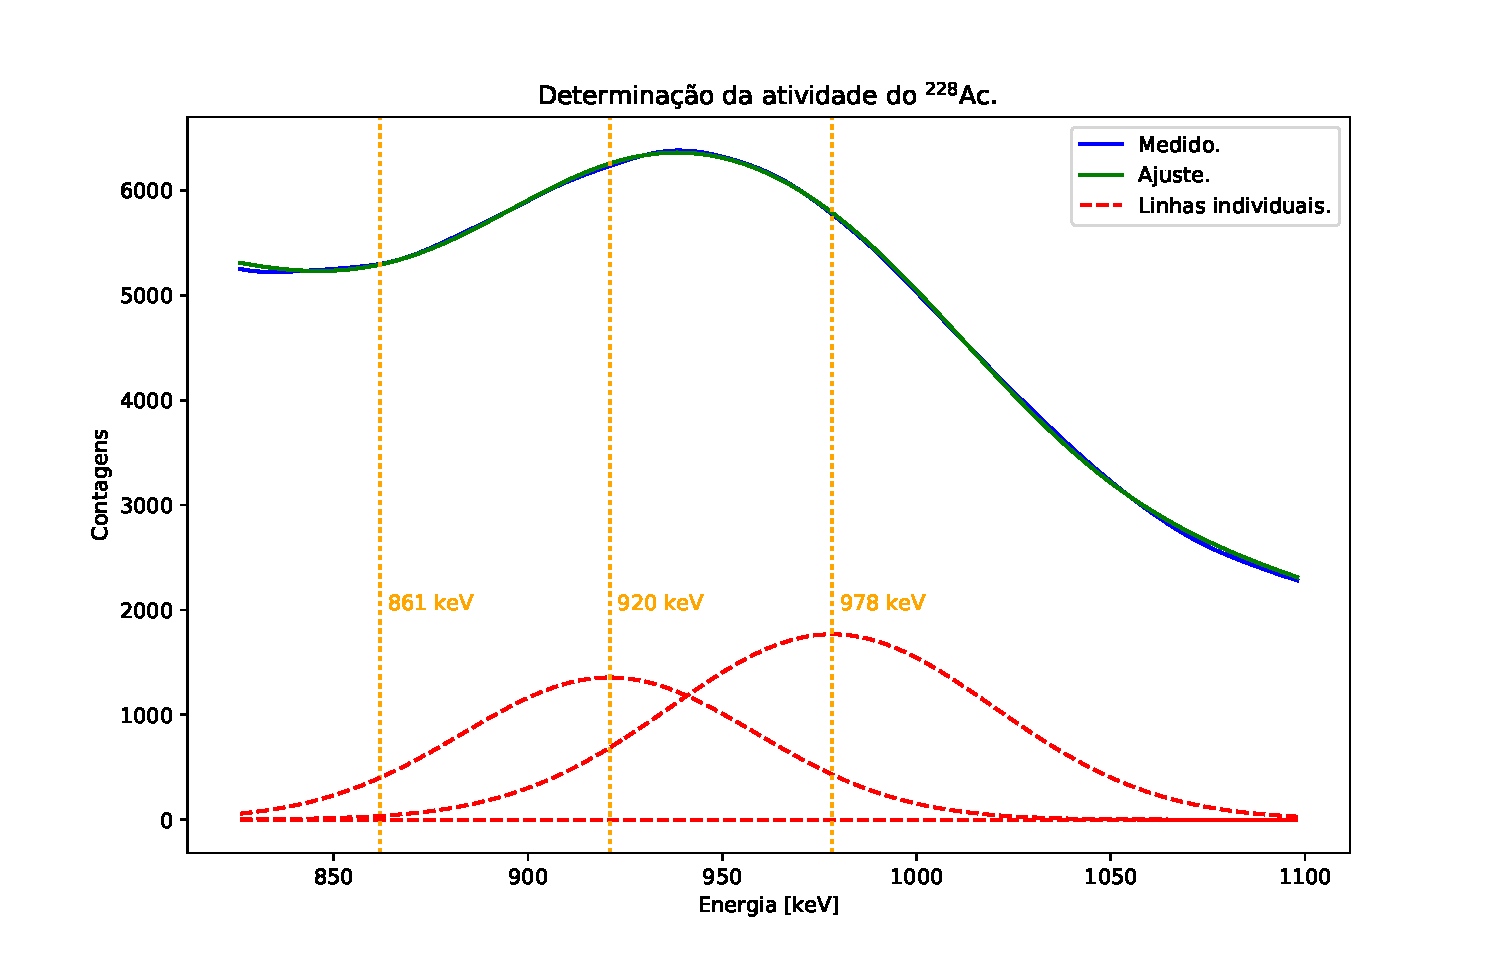
\includegraphics[width=0.9\textwidth]{atividade_ac.pdf}
  \caption{Determinação da atividade do ${}^{228}$Ac.}
  \label{fig:atividade.ac}
\end{figure}

Determinamos então a intensidade das emissões do Actínio na janela de observação\footnote{Esta intensidade corresponde ao número de contagens devidas ao Actínio esperadas na região da janela de observação se o detector possuísse eficiência uniforme igual à eficiência em 240 keV.} segundo a equação \eqref{eq:i_Ac}, obtendo

\[i_{Ac} = 49000 \pm 6000 \]

Com os dados das tabelas de radionuclídeos \cite{TabRad_v6}, encontramos que a probabilidade de uma emissão aleatória do ${}^{228}$Ac ocorrer com energia entre $825$ e $1100$ keV é de

\[ p_{Ac} = 8.15 \% \]

Portanto, utilizando a expressão \eqref{eq:I_Ac} encontramos que a atividade do ${}^{228}$Ac é de

\[ I_{Ac} = 600000 \pm 70000 \]

Para determinar a atividade do ${}^{212}$Th, ajustamos a função \eqref{eq:um.pico} aos dados obtidos (o gráfico do ajuste pode ser visto na Figura \ref{fig:atividade.pb}). Os valores obtidos do ajuste para a amplitude e média da gaussiana foram

\begin{figure}[H]
  \centering
  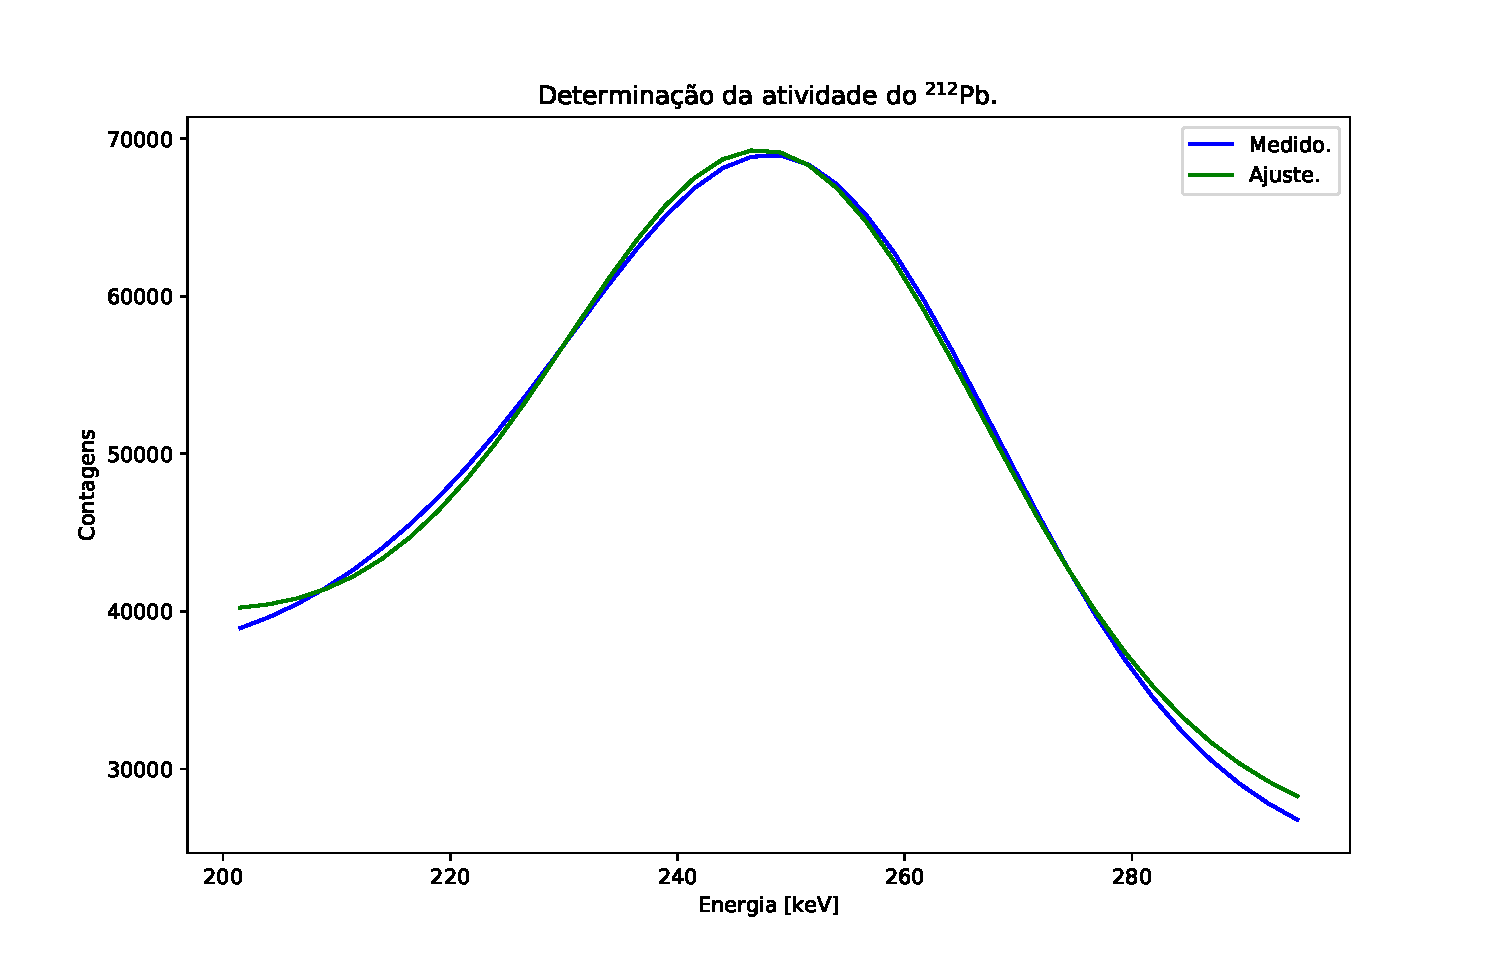
\includegraphics[width=0.9\textwidth]{atividade_pb.pdf}
  \caption{Determinação da atividade do ${}^{212}$Pb.}
  \label{fig:atividade.pb}
\end{figure}

\[ A_1 = 170000 \pm 10000 \]
\[ E_1 = 248.5 \pm 0.1 \text{keV} \]

A intensidade das emissões do ${}^{212}$Pb na região entre 200 e 295 keV, corrigida pela eficiência do detector, é, portanto,

\[i_{Pb} = 28400 \pm 200 \]

Utilizando os dados da tabela de radionuclídios \cite{TabRad_v2}, obtemos que a probabilidade de uma transição do ${}^{212}$Pb ocorrer entre 200 e 295 keV é de

\[ p = 43.6 \% \]

Portanto a atividade do ${}^{212}$Pb é de

\[I_{Pb} = 65100 \pm 400 \]

Finalmente, obtemos que a razão das atividades do ${}^{228}$Ra e do ${}^{228}$Th é de

\[ r = \frac{A_{Ra}}{A_{Th}} = \frac{I_{Ac}}{I_{Pb}} \]
\[ r = 1.4 \pm 0.2 \]

Encontrando as raízes da função $f(t) = r(t) - r$, onde $r(t)$ é dada pela equação \eqref{eq:razao.teorica}, encontramos que a idade da amostra é

\[ t = 2.2 \pm 0.1 \text{ anos.} \]

\section{Conclusão}

Experimentos utilizando espectrômetro gama possibilitam uma boa introdução à Física Nuclear, sendo possível observar o papel dos detectores e da instrumentação nas medidas, a verificação de vários modelos importantes da Física Moderna, como a relatividade especial e o espalhamento Compton e também algumas questões ligadas à análise de dados propriamente dita, e o papel da estatística em extrair resultados de conjuntos grandes de dados.

Observamos, por fim, que todos os scripts e dados utilizados para a análise são públicos e licenciados sob GPL v3\footnote{\url{https://www.gnu.org/licenses/gpl.html}}, estando disponíveis para consulta e utilização em \url{https://github.com/prcaetano/Espectroscopia-Gama/}, de forma que toda a análise aqui descrita é reprodutível por terceiros.

\printbibliography

\end{document}
